%\paragraph{\bf Abstract.}
%\keywords{conditionally lexicographic preferences, social choice theory,
%positional scoring voting rules, answer set programming}
Aggregating \emph{votes} --- preference orders over \emph{candidates} 
or \emph{alternatives} --- is a fundamental problem of decision theory 
and social choice. We study this problem in the setting when 
alternatives are described as tuples of values of attributes. Such spaces of 
alternatives are called \emph{combinatorial}. They are characterized by 
large sizes that make explicit enumerations of alternatives from the most 
to the least preferred infeasible. Instead, typically votes are specified 
implicitly 
in terms of some compact and intuitive preference representation mechanism. 
In our work, we assume that votes are given as \textit{lexicographic 
preference trees} and consider two preference-aggregation problems, the 
\emph{winner} problem and the \emph{evaluation} problem. We study them 
under the assumption that \textit{positional scoring rules} (such as 
$k$-approval and Borda) are used for aggregation. We develop computational 
complexity results for these two problems. We also propose computational 
methods to solve 
them. They are based on encodings of the problems in \textit{Answer-Set 
Programming} and as instances of the \textit{Weighted Partial Maximum 
Satisfiability} problem, and exploit off-the-shelf solvers available for 
these two formalisms. Finally, we present results of an experimental study 
of the effectiveness of these methods.

\section{Introduction}
Preferences are an essential component of decision making, social choice,
knowledge representation, and constraint satisfaction. Fundamental 
problems of preference reasoning are to \emph{aggregate} individual 
preference orders of a group of agents (the \emph{votes} of agents in 
the group) into a consensus best candidate (the \emph{winner}), and to 
identify candidates with strong consensus support from the group 
(``good'' alternatives). These problems
have been studied extensively in social choice \cite{arrowhandbook}. 
Aggregation methods known as \emph{positional scoring rules}, which include
such well-known rules as plurality, $k$-approval and Borda, are
among the best understood and the most widely used ones.
 
When the number of alternatives is small, the simplest and most effective 
way to describe a preference order (a vote) is to enumerate the
alternatives from the most to the least preferred. Moreover, given a 
collection of such votes, for many aggregation rules, including all 
positional scoring rules, computing winners and ``good'' candidates is 
easy --- it can be done in polynomial time. The situation changes when
alternatives are characterized in terms of \emph{attributes} (or issues),
and are specified by tuples of attribute values. Spaces of such alternatives,
often called \emph{combinatorial domains}, are large. Indeed, the number 
of alternatives grows exponentially with the number of attributes. This
large size of combinatorial domains brings up two problems. First, it is
no longer feasible to describe votes by enumerating alternatives in the
order of preference. Thus, formalisms offering compact and intuitive
representations of votes are needed. Several such \emph{preference
formalisms} have been developed over the years including penalty logic 
\cite{de1994penalty}, possibilistic logic \cite{DuboisLP91}, conditional
preference networks (CP nets) \cite{bbdh03}, preference
trees \cite{fraser1994ordinal,liu2015reasoning}, 
and lexicographic preference trees \cite{booth:learningLP}.%
\footnote{Kaci \cite{Kaci:Pref} offers a comprehensive discussion of 
preference formalisms.} Second, when votes are given as expressions in 
some preference formalism, computing the winner or a ``good'' candidate 
is no longer easy. In fact, it is known that for many preference formalisms 
these problems are NP-hard even when positional scoring rules are used 
to aggregate votes. \emph{Issue-by-attribute} aggregation addresses the
computational hardness problem but often leads to results different from 
those obtained by applying common voting rules \cite{fargier:ibi}.
  
In this chapter, we assume that votes are represented as \emph{lexicographic
preference trees}, or \emph{LP-trees}, for short~\cite{booth:learningLP},
and that they are aggregated by some simple positional scoring rules such 
as Borda, $k$-approval and a refinement of the latter, $(k,l)$-approval.
Given this setting, we study computing the best alternative, and the related 
problem to decide whether an alternative with the score exceeding a given 
threshold (a ``good'' alternative) exists. We refer to the former problem 
as the \emph{winner} problem and to the latter one as 
the \emph{evaluation} problem. In our setting, these problems are often
computationally hard. For Borda, the \emph{winner} problem is NP-hard and 
the \emph{evaluation} problem is NP-complete \cite{lang:aggLP}. For $k$-approval, 
for some specific values of $k$, both problems are in P but, for some other, 
they are NP-hard and NP-complete, respectively \cite{lang:aggLP}. Further,
when $(k,l)$-approval is used, for several values 
of $k$ and $l$, the problems are similarly hard.

Nevertheless, because the \emph{winner} and the \emph{evaluation}
problems arise in practice and the positional scoring rules
are common, computational tools for the two problems are needed. To 
develop such tools, we encode the problems in answer-set programming (ASP) 
\cite{mt99:stable,Niemela:1999} and weighted partial maximum satisfiability 
(WPM-SAT) \cite{ansotegui2010new,ansotegui2009solving}, and apply to the 
encodings the ASP solvers \emph{clingo} \cite{Gebser:clingo} and 
\emph{clingcon} \cite{Ostrowski:clingcon}, and a WPM-SAT solver \toulbar 
\cite{toulbar2}. We chose the two ASP solvers as they represent substantially
different approaches to computing answer sets. The \emph{clingo} solver is 
a native ASP solver developed along the lines of satisfiability solvers. 
The \emph{clingcon} solvers enhances \emph{clingo} with specialized 
treatment of some common classes of numeric constraints by delegating some 
reasoning tasks to a CP solver \emph{Gecode}~\cite{Schulte:gecode}. As 
problems we are considering involve numeric constraints, a comparison of 
the two solvers is of interest. We study all the resulting methods 
experimentally. To support the experimentation we propose and implement 
a method to randomly generate LP-trees of some restricted form.

The main contributions of our work are complexity results and algorithms 
for the \emph{winner} and the \emph{evaluation} problems when votes are 
specified as LP-trees. Specifically, we present new complexity results 
for the two problems for several positional scoring rules: $k$-approval 
(for specific values of $k$), variants of Borda, and $(k,l)$-approval 
(for specific combinations of values of $k$ and $l$). Next, we propose
algorithms for the two problems based on their ASP and WPM-SAT encodings 
and using ASP and WPM-SAT solvers. Finally, we provide an experimental 
evidence of the effectiveness of the proposed computational methods.


\section{Computing Ranks}
We now show how the \tit{rank} of an outcome in an LP-tree is computed.
As we consider positional scoring rules, the scores of an outcome
in an LP-tree or an LP-profile under these rules follow directly
from its rank in the tree.

Given an LP-tree $T$ and an outcome $o\in \CD(\cI)$,
the computation of the rank $r(T,o)$ of $o$ in $T$
is given in \algref{rank}, where $T'(x_j)$ is the 
left (more-preferred) subtree of $T'$, and
$T'(\obar{x_j})$ is the right (less-preferred)
subtree of $T'$. Note that in each case we need to
update the CPT's in the subtrees accordingly.
Clearly, \algref{rank} takes $O(p)$.
Conversely, it is also easy to compute the outcome
at a given rank in a tree.

\begin{algorithm}
\KwIn{LP-tree $T$ and outcome $o$}
\KwOut{the rank $r$ of $o$ in $T$}
	$r \lar 0$\;
	$T' \lar T$\;
	\For{$i \lar 1$ \KwTo $p$}{
		Let $X_j$ be the root attribute of $T'$ with preference $x_j > \obar{x_j}$\;
		\uIf{$o(X_j) = x_j$}{
			$T' \lar T'(x_j)$\;
		}
		\Else{
			$r \lar r + 2^{p-i}$\;
			$T' \lar T'(\obar{x_j})$\;
		}
	}
	\Return{$r$}
\caption{Compute the rank of an outcome in an LP-tree\label{alg:rank}}
\end{algorithm}

Now computing the scores of an outcome for the rules
$k$-approval, $(k,l)$-approval and Borda is straightforward.
We have the following.
\begin{enumerate}
	\item $k$-approval: $s_\kApp(T,o)=1$, if $r(T,o)<k$; $0$, otherwise.
	\item $(k,l)$-approval: $s_\klApp(T,o)=a$, if $r(T,o)<k$; $b$, if $k\leq r(T,o)<k+l$;
				$0$, otherwise.
	\item Borda: $s_\Borda(T,o)=m-r(T,o)-1$.
\end{enumerate}


\section{The Problems and Their Complexity}

We consider only \emph{effective implicit} positional scoring rules, 
that is, rules defined by an algorithm that given $m$ (the number of 
alternatives and, at the same time, the size of the scoring vector) 
and a rank $r$, $0\leq r\leq m-1$, (1) returns the value $w_r$ of 
the scoring vector, and (2) works in time polynomial in the sizes of 
$r$ and $m$. The rules $k$-approval, $(k,l)$-approval and Borda are examples 
of effective implicit positional scoring rules:

\begin{enumerate}
	\item $k$-approval: $w_\kApp(r,m)=1$, if $r<k$; $0$, otherwise.
	\item $(k,l)$-approval: $w_\klApp(r,m)=a$, if $r<k$; $b$, if $k\leq r<k+l$;
				$0$, otherwise.
	\item Borda: $w_\Borda(r,m)=m-r-1$.
\end{enumerate}

Let us fix an effective implicit positional scoring rule $\cD$ with the
scoring vector $w$. Given an LP profile $\cV$, the \emph{winner} problem for
$\cD$ consists of computing an alternative $o \in \cX$ with the maximum 
score $s_w(\cV,o)$. Similarly, given a profile $\cV$ and a positive integer 
$R$, the \emph{evaluation} problem for $\cD$ asks if there exists an 
alternative $o \in \mathcal{X}$ such that $s_{{w}}(\cV, o)\geq R$. In 
each case, $w$ is the scoring vector of $\cD$ for $m$ alternatives; we recall
that it is given implicitly in term of an algorithm that efficiently 
computes its entries.
     
We apply the voting rules listed above to profiles consisting of LP-trees or
\emph{LP profiles}, for short. We distinguish four classes of profiles,
UI-UP, UI-CP, CI-UP and CI-CP depending on the type of LP-trees they
consist of. 

\begin{remark}
The restriction to effective implicit positional scoring rules is 
essential in the context of combinatorial domains. It is because an 
explicit specification of the scoring vector has size equal to the 
number of alternatives and is exponential in the number of attributes. If 
it were to be given explicitly, it would have to be a part of input. 
The sheer size of the scoring vector would then make both the winner 
and the evaluation problems trivially solvable in polynomial time. 
However, most interesting positional scoring rules are effective 
implicit, which means that they can be described concisely as an 
algorithm (implicit) and at the same time provide a fast access to 
any weight in the scoring vector (effective). In this setting, the 
complexity of the winner and the evaluation problems is no longer 
obvious, and it is precisely this setting that models practical
situations, where scoring vectors are based on \emph{regular}
patterns.
\end{remark}


\subsection{$k$-Approval}
If $k=2^{p-1}$ the evaluation problem is in P for all four classes of 
profiles of LP-trees \cite{lang:aggLP}. However, if $k$ equals $2^{p-2}$
or $2^{p-3}$, the problem is NP-complete, again for all four types of 
profiles \cite{lang:aggLP} (in fact, the result holds for a larger set 
of values $k$, we refer for details to the paper by Lang et al. 
\cite{lang:aggLP}). Clearly, in each case where the evaluation problem 
is NP-complete, the winner problem is NP-hard.

We first show that the two problems are in P even when the deviation of
$k$ from $2^{p-1}$ is given by a polynomial in $p$. In other words, 
if $k=2^{p-1} + f(p)$ or $k=2^{p-1} - f(p)$, where $f(p)$ is a polynomial 
in $p$ such that $f(p)\geq 0$ for $p\geq 1$, both the winner and the 
evaluation problems for $k$-approval can be solved by polynomial time 
algorithms. The next two results address the two cases for $k$,
respectively.

\begin{thm}
\label{thm1}
Let $f$ be a polynomial such that $f(p)\geq 0$ for $p\geq 1$, and let
$k=2^{p-1}+f(p)$. Given 
a profile of $n$ LP-trees over $p$ binary attributes $X_1,\ldots,X_p$, the 
winner under $k$-approval can be computed in time polynomial in the
size of the profile.
\end{thm}
\begin{proof}
Let $P$ be a profile of $n$ LP-trees. The score $s_k(o)$ of an alternative
$o$ under $k$-approval in $P$ is given by 
\[
s_k(o) = s'(o)+s''(o),
\]
where $s'(o)$ is the score of $o$ under the $2^{p-1}$-approval (the number
of votes that place $o$ in the upper half of the order), and $s''(o)$ is the
number of votes that place $o$ as one of top $f(p)$ votes in the lower 
half (we omit references to the profile to simplify the notation).

To find the highest possible score $s'(o)$, we define $x_i=0$, if 
the number of votes with the root labeled with $X_i$ and with 0 preferred
to 1 is \emph{strictly} larger than the number of votes with the root 
labeled with $X_i$ with 1 preferred to 0. We define $x_i=1$ similarly.
If $x_i$ does not get set to 0 or 1, it is set to $u$ (undefined). We
call the resulting $p$-tuple a \emph{partial alternative} and denote 
it by $PA$. Since it is the root that decides whether an LP-tree 
contributes 1 to the score of an alternative, it is clear that any 
alternative consistent with $PA$ achieves the highest possible 
score under $2^{p-1}$-approval, that is, the highest possible $s'$-score.  
Finding this score, say $W'$, can then be accomplished by (1) finding
an alternative $o$ consistent with $PA$, and (2) finding its score $s'(o)$.
Clearly, both (1) and (2) together can be done in time bounded by a polynomial 
in the size of the profile.

Next, we consider $s''$. Let us denote by $A$ the set of all alternatives 
$o$ with $s''(o)>0$. To this end, it is enough
to find in each tree $T$ in $P$ alternatives with ranks $2^{p-1}+1,
\ldots, 2^{p-1}+f(p)$. Since finding an alternative of a given rank in 
an LP-tree can be accomplished in time polynomial in $p$, the set $A$ 
can indeed be computed in time polynomial in the size of the profile.

We now compute $s_k(o)$ for all alternatives in $A$. Given the size of
$A$, the task can be computed in time bounded by a polynomial in the size
of the profile. Let $W$ be the maximum of these scores achieved, say, by an
alternative $o$. If $W\geq W'$, then $o$ is a winning alternative (has 
the best score among those in $A$ and the score of any other alternative 
does not exceed $W'$). Otherwise, any alternative consistent with $PA$ 
can be taken for the winner (indeed, in such case, the highest possible 
score to achieve under $k$-approval is $W'$). 
\end{proof}

%\begin{cor}
	%Theorem \ref{thm1} holds for $k$-approval when 
	%$k=2^{p-1}+f(p)$, where $f(p)$ is a polynomial in $p$.
%\end{cor}

\begin{thm}
\label{thm2}
Let $f$ be a polynomial such that $f(p)\geq 0$ for $p\geq 1$, and let
$k=2^{p-1}-f(p)$. Given a profile of $n$ LP-trees over $p$ binary attributes 
$X_1,\ldots,X_p$, the winner under $k$-approval can be computed in time 
polynomial in the size of the profile.
\end{thm}
\begin{proof}
Let $P$ be a profile of $n$ LP-trees. Similarly as in the proof of the
previous result, the score $s_k(o)$ of an alternative $o$ under 
$k$-approval is given by
\[
s_k(o) = s'(o)-s''(o),
\]
where $s'(o)$ is the score of $o$ under the $2^{p-1}$-approval (the number
of votes that place $o$ in the upper half of the order), and $s''(o)$ is the
number of votes that place $o$ as one of the bottom $f(p)$ votes in the upper
half (we omit references to the profile to simplify the notation).

Let us denote by $A$ the set of alternatives $o$ such that $s''(o)>0$.
As before, this set can be computed in time bounded by a polynomial in 
the size of the profile. Let $t=|A|$. If every alternative is in $A$
(that is, $t=2^p$), then, we compute an alternative with the highest
$k$-approval score by computing the scores of all alternatives in $A$
and selecting the one with the highest score. Since the size of $A$ is
polynomial in the size of the profile, the task takes polynomial time
(in the size of the profile).

The case when $t< 2^p$ is harder. To address it, let us assume that we 
have computed the set $B$ of top $t+1$ alternatives according to their 
$s'$-score (the $2^{p-1}$-approval score). Next, let $o$ be an alternative 
in $B$ with the maximum $k$-approval score $s_k(o)$.

We claim that $o$ is also an alternative with the maximum $k$-approval 
score over all alternatives. Indeed, consider an arbitrary alternative 
$o'$. If $o'\in B$, then $s_k(o)\geq s_k(o)$ (by the way $o$ was selected). 
Thus, let us assume that $o'\notin B$. Since $|B|> |A|$, there is at least 
one alternative $o''\in B\setminus A$. As $o''\in B$, $s_k(o)\geq s_k(o'')$.
Moreover, as $o''\notin A$, $s_k(o'')=s'(o'')-s''(o'')=s'(o'')$. Finally,
since $o''\in B$ and $o'\notin B$, $s'(o'')\geq s'(o')$. Combining these 
three inequalities, we obtain that $s_k(o) \geq s'(o')$. Since $s'(o')\geq 
s'(o')-s'(o'')=s_k(o')$, we get $s_k(o)\geq s_k(o')$. Thus, the claim follows.

Clearly, $t+1$ is bounded by a polynomial in the size of the profile. 
Thus, once $B$ is computed, finding an alternative in $B$ with the 
highest $k$-approval score can be done in time polynomial in the size 
of the profile. To complete the proof, it suffices then to show how to 
compute $B$ in polynomial time. 

To this end, for each $i=1,\ldots,p$, we set $d_i$ to the absolute value 
of the difference between the numbers of trees in the profile with the root 
labeled with $X_i$ and with 0 (respectively, with 1) as the preferred value. 
We also select any alternative that has the highest $s'$-score (we 
explained in the previous proof how to compute it in polynomial time)
and denote it by $o$. Finally, we compute the score of $o$ and denote it 
by $W'$ (to use the notation from the previous proof). 

Let $S\subseteq\{1,\ldots,p\}$ be a set of attribute indices, and let $o_S$
be an alternative obtained from $o$ by ``flipping'' its values in 
positions in $S$. Every alternative can be described in these terms.
This is useful as the $s'$-score of $o_S$ is easy to compute. Namely, 
we have
\[
s'(o_S) = W' - w(S),
\]
where $w(S)=\sum_{i\in S} d_i$ is the \emph{weight} of $S$.

It follows that $B$ is determined by $t+1$ smallest-weight subsets 
of $\{1,\ldots,p\}$. We will now show that given a list $D=\{d_1,d_2,
\ldots,d_p\}$ and an integer $t$, the $t+1$ smallest-weight subsets 
of $\{1,\ldots,p\}$ can be computed in time bounded by a polynomial in
$p$ and $t$.  

Let $r$ be an integer such that $2^r\geq t+1$. Let us assume that $L_r$ is
the set of $t+1$ smallest-weight subsets of $\{1,\ldots,r\}$. Let 
\[
L'_{r+1}=L_r \cup \{S\cup \{r+1\}\colon S\in L_r\}
\]
and let $L_{r+1}$ be the collection of $t+1$ smallest-weight subsets $S$
of $L'_{r+1}$. We will show that $L_{r+1}$ contains $t+1$ smallest-weight 
subsets $S$ of $\{1,\ldots,r+1\}$. Indeed, let us consider $S\subseteq\{1,
\ldots,r+1\}$ such that $S\notin L'_{r+1}$. If $S\subseteq \{1,\ldots, r\}$,
then $S\notin L_r$. Thus, $w(S)\geq w(S')$, for every $S'\in L_r$.
If $r+1\in S$, then $S=R\cup\{r+1\}$, for some $R\subseteq \{1,\ldots,r\}$.
Since $S\notin L'_{r+1}$, $R\notin L_r$. Thus, $w(R)\geq w(R')$, for every
$R'\in L_r$ and so, $w(S)\geq w(R'\cup\{r+1\})$ for all $R'\in L_r$.
In each case, it follows that there are at least $t+1$ sets $S'$ in 
$L'_{r+1}$ such that $w(S)\geq w(S')$. Thus for every $S'\in L_{r+1}$, 
$w(S)\geq w(S')$. 

Clearly, the list $L_p$ consists of $t+1$ smallest weight subsets of
$\{1,\ldots,p\}$. Thus, it can be taken for $B$. To compute it, we first
find the smallest $r$ such that $2^r\geq t+1$ (such an $r$ exists as
we are now considering the case when $t < 2^p$). We then construct the 
collection $U$ of all subsets of $\{1,\ldots, r\}$ (this collection 
has no more than $2t$ elements and can be constructed in time bounded 
by a polynomial in $p$ and $t$). Next, we construct $L_r$ by selecting 
from $U$ its $t+1$ smallest-weight elements. Since $|U|\leq 2t$, this task
also can be accomplish in polynomial time (in $p$ and $t$).

From now on, we construct $L_{r+1},L_{r+2},\ldots L_p$ recursively, as 
described above. Since each step of the construction can be accomplished
by the same polynomial-time algorithm (form the collection $L'$, select
its $t+1$ smallest-weight elements to form the next $L$), and since
the number of steps is bounded by $p$, the total time needed to construct
$B$ ($L_p$) is bounded by a polynomial in $p$ and $t$.  
\end{proof}

%\begin{cor}
	%Theorem \ref{thm2} holds for $k$-approval when 
	%$k=2^{p-1}-f(p)$, where $f(p)$ is a polynomial in $p$.
%\end{cor}

For the $k$-approval rule, we summarize the results in \tblref{kApp_comp},
where \tblref{kApp_comp_a} presents our results as discussed above,
and results in \tblref{kApp_comp_b} were obtained by others
\cite{lang:aggLP}.
\begin{table}
	\centering
	\caption{$k$-Approval}
  \begin{subfigure}[b]{0.5\textwidth}
		\centering
		\begin{tabular}[0.5\textwidth]{ | c | c | c | }
		  \hline
		    & UP & CP \\
		  \hline
		  UI & P & P \\
		  \hline
		  CI & P & P \\
		  \hline
		\end{tabular}
		\caption{$k=2^{p-1}\pm f(p)$}
		\label{tbl:kApp_comp_a}
	\end{subfigure}%
  \begin{subfigure}[b]{0.5\textwidth}
		\centering
		\begin{tabular}[0.5\textwidth]{ | c | c | c | }
		  \hline
		    & UP & CP \\
		  \hline
		  UI & NPC & NPC \\
		  \hline
		  CI & NPC & NPC \\
		  \hline
		\end{tabular}
		\caption{$k=c\cdot 2^{p-M}$ and $k \not = 2^{p-1}$}
		\label{tbl:kApp_comp_b}
	\end{subfigure}
	\label{tbl:kApp_comp}
\end{table}


\subsection{$(k,l)$-Approval}
%In the most restrictive case of UI-UP profiles, the evaluation
%problem for the Borda rule is in P and it is NP-complete for the three
%other classes of profiles \cite{lang:aggLP}. The picture for the 
%the $k$-approval rule is more complicated. If $k=2^{p-1}$ the evaluation
%problem is in P for all four classes of profiles. 
%However, if $k$ equals $2^{p-2}$ or $2^{p-3}$,
%the problem is NP-complete, again for all four LP profile types
%\cite{lang:aggLP} (in fact, the result holds for a larger set of values
%$k$, we refer for details to Lang et al. \cite{lang:aggLP}).
%Clearly, in each case where the evaluation problem is NP-complete, the winner
%problem is NP-hard.

To the best of our knowledge, the complexity of the 2-valued $(k,l)$-approval 
rule has not been studied. It is evident that $(k,l)$-approval is an effective
implicit positional scoring rule. It turns out that, as with the $k$-approval 
rule, for some values of the parameters, the evaluation problem for 
$(k,l)$-approval is NP-complete. Preliminary results we obtained 
have been published \cite{conf/adt13/LiuT}.
We describe cases where $k=l=2^{p-c}$,
where $c$ is a constant and $1<c<p$.
%We describe two such cases here: (1) $k=l=2^{p-2}$, and (2) $k=l=2^{p-3}$.
%We note that if $a=1$ and $b=0$, case (1) reduces to $2^{p-2}$-approval 
%and case (2) to $2^{p-3}$-approval. 
If $a=2$ and $b=1$, we refer to the rule 
$(2^{p-2},2^{p-2})$-approval as $2K$-$approval$.
We show proof of NP-completeness of the evaluation problem for
$(2^{p-2},2^{p-2})$-approval.

\begin{thm}
The following problem is NP-complete: decide for a given UI-UP profile 
$\cV$ and an integer $R$ whether there is an alternative $o$ such that 
$s_w(\cV,o) \geq R$, where $w$ is the scoring vector of the $(2^{p-2},
2^{p-2})$-approval rule.
\end{thm}
\begin{proof}
        We can guess in polynomial time an alternative $o \in \mathcal{X}$ and
        verify in polynomial time that $S_w(\cV, o) \geq R$ (this is possible 
because $(k,l)$-approval is an effective implicit scoring rule; the score of an alternative in
a vote can be computed in polynomial time once its position is known, and 
the position can be computed in polynomial time be traversing the tree 
representing the vote).  So membership in NP follows.
        Hardness follows from a polynomial reduction from the
        problem $2$\textit{-MINSAT}\footnote{Let $N$ be an integer ($N>1$),
				the $N$-MINSAT problem
        is defined as follows.  Given a set $\Phi$ of $n$ $N$-clauses
        $\{ c_1,\ldots,c_n \}$ over a set of propositional variables
        $\{ X_1,\ldots,X_p \}$,
        and a positive
        integer $l$ ($l \leq n$), decide whether there is a truth assignment that
        satisfies at most $l$ clauses in $\Phi$.} \cite{Kohli:2maxsat}, which is NP-complete.
        Given an instance $\langle \Phi, l \rangle$ of the 2-MINSAT problem,
we construct the set of attributes
        $\cI$, the set of alternatives $\mathcal{X}$, the profile $\cV$ and the threshold $R$.

        Important observations are that $o$ is among the
				top first quarter of alternatives in an LP-tree 
$\mathcal{L}$ if and only if the top two most important attributes in $\mathcal{L}$ 
are both assigned the preferred values; and that $o$ is among the second top 
quarter of alternatives if and only if the most important attribute is assigned 
the preferred value and the second most important one is assigned the 
non-preferred one.
				
\noindent
(1). We define $\cI = \{ X_1,\ldots,X_p \}$, where $X_i$s are all propositional
letters occurring in $\Phi$. Clearly, the set $\cX$ of all alternatives over 
$\cI$ coincides with the set of truth assignments of variables in $\cI$.

\noindent
(2). Let $\Psi$ be the set of formulas $\{ \neg c_i:c_i \in \Phi \}$.  
For each $\neg c_i \in \Psi$, we build $a+b$ UI-UP trees. For instance, 
if $\neg c_i = X_2 \land \neg X_4$, then we proceed as follows.
Firstly, we build $a-b$ duplicate trees shown in
\figref{proof1}. Secondly, we construct $b$ duplicate trees shown in
\figref{proof2}. Thirdly, we build another $b$ duplicate trees shown in
\figref{proof3}. (In all three figures we only indicate the top two attributes 
since the other attributes can be ordered arbitrarily.) Denote by $\cV_i$ the 
set of these $a+b$ UI-UP trees for formula $\neg c_i$. Then $\cV = \bigcup_{1 
\leq i \leq n} \cV_i$ and has $n*(a+b)$ votes.

\noindent
(3). Finally, we set $R=(n-l)*(a^2-ab+b^2)+l*ab$.

        Note that the construction of $\cV$ ensures that if $o \models \neg c_i$, $S_w(\cV_i, o)=
        a^2-ab+b^2$; 
				otherwise if $o \not \models \neg c_i$, $S_w(\cV_i, o)=ab$.  We have $a^2-ab+b^2 > ab$ since 
        $(a-b)^2 > 0$.  Hence, there is an assignment 
				satisfying at most $l$ clauses in $\Phi$ 
if and only if there is an assignment satisfying 
				at least $n-l$ formulas in $\Psi$ 
if and only if there is an alternative with the $(2^{p-2},2^{p-2})$-approval
score of at least $R$ given the profile $\cV$. 

Since the first equivalence is clear, it suffices to show the second.
Let $o$ be an assignment satisfying $l'$ formulas in $\Psi$. 
We have $S_w(\cV, o) - R = (l'+l-n)*(a^2-ab+b^2)+(n-l'-l)*ab
= (l'+l-n)*(a^2-2ab+b^2) = (l'+l-n)*(a-b)^2$.
It follows that $S_w(\cV, o) \geq R$ if and only if $l'+l-n \geq 0$
if and only if $l' \geq n-l$.  
\end{proof}

\begin{figure*}[!ht]
  \centering
  \setlength{\tabcolsep}{0mm}
  \begin{tabular}{c}
  \begin{subfigure}[b]{0.25\textwidth}
    \begin{tikzpicture}[->,>=stealth',node distance=1.5cm,main node/.style={circle,draw,font=\small}]
      \node[main node] (1) {$X_2$};
      \node[rectangle,draw] at (1.3,0) {$1_2 > 0_2$};

      \node[main node] (2) [below of=1] {$X_4$};
      \node[rectangle,draw] at (1.3,-1.5) {$0_4 > 1_4$};

      \path[]
        (1) edge (2);
    \end{tikzpicture}
    \caption{}
    \label{fig:proof1}
  \end{subfigure}

  \begin{subfigure}[b]{0.25\textwidth}
    \begin{tikzpicture}[->,>=stealth',node distance=1.5cm,main node/.style={circle,draw,font=\small}]
      \node[main node] (1) {$X_4$};
      \node[rectangle,draw] at (1.3,0) {$1_4 > 0_4$};

      \node[main node] (2) [below of=1] {$X_2$};
      \node[rectangle,draw] at (1.3,-1.5) {$0_2 > 1_2$};

      \path[]
        (1) edge (2);
    \end{tikzpicture}
    \caption{}
    \label{fig:proof2}
  \end{subfigure}

  \begin{subfigure}[b]{0.25\textwidth}
    \begin{tikzpicture}[->,>=stealth',node distance=1.5cm,main node/.style={circle,draw,font=\small}]
      \node[main node] (1) {$X_4$};
      \node[rectangle,draw] at (1.3,0) {$0_4 > 1_4$};

      \node[main node] (2) [below of=1] {$X_2$};
      \node[rectangle,draw] at (1.3,-1.5) {$0_2 > 1_2$};

      \path[]
        (1) edge (2);
    \end{tikzpicture}
    \caption{}
    \label{fig:proof3}
  \end{subfigure}
  \end{tabular}

  \caption{UI-UP LP-trees}
  \label{fig}
\end{figure*}

This hardness proof applies to more general classes of LP-trees, namely 
UI-CP, CI-UP and CI-CP, and the winner problem for those cases is NP-hard.
%In general, the evaluation problem according to $(2^{p-c},2^{p-c})$-approval,
%where $c$ is a constant and $1<c<p$, for the four 
%classes of LP-trees is NP-complete. In each case, the hardness follows from
%from an NP-complete version of the \textit{c-MINSAT} problem. 
Below we show the proof of NP-completeness of the evaluation problem
for $(2^{p-3},2^{p-3})$-approval.

\begin{thm}
	Let $w$ be the scoring vector $(a,\ldots,a, b,\ldots,b, 0\ldots,0)$ with the numbers of 
	$a$'s and $b$'s each equal to $2^{p-3}$.  The problem of deciding for a given UI-UP profile 
	$V$ and an integer $R$ whether there is an alternative
	$o$ such that $s_w(V,o) \geq R$ is NP-complete.
\end{thm}
\begin{proof}
  We can guess in polynomial time an alternative $o \in \mathcal{X}$ and 
  verify in polynomial time that $S_w(V, o) \geq R$.  So membership in NP follows.

  Hardness follows from a polynomial reduction from the NP-complete 
  problem 3\textit{-MAXSAT} \cite{Papadimitriou:1988}.
  Let $\Phi$ be a set of $n$ 3-clauses $\{ c_1,\ldots,c_n \}$ over $\{ X_1,\ldots,X_p \}$, 
  $l$ an integer such that $0 \leq l \leq n$.
  Given an instance of 3\textit{-MAXSAT} $I=\langle \Phi, l \rangle$, we construct the set of attributes 
  $X$, the set of alternatives $\mathcal{X}$, the profile $V$ and the threshold $R$ as follows.

  (1) $X = \{ X_1,\ldots,X_p \}$.  $\mathcal{X}$ is then the set of 
      all alternatives over $X$.

  (2) Let $\Psi$ be the set of formulas $\{ \neg c_i:c_i \in \Phi \}$.  For each 
      $\neg c_i \in \Psi$, we build multiple UI-UP LP-trees.  Assume there is $c_i = 
      \neg X_1 \vee \neg X_2 \vee \neg X_3 \in \Phi$. Then we have $\neg c_i = X_1 \wedge 
      X_2 \wedge X_3 \in \Psi$.  For $\neg c_i$, we build $a^2$ duplicate trees of 
      type~\ref{fig:1}, $a^2$ duplicate trees of type~\ref{fig:2}, $a^2$ duplicate 
      trees of type~\ref{fig:3}, $a^2$ duplicate trees of type~\ref{fig:4}, 
      $a^2-ab$ duplicate trees of type~\ref{fig:5}, 
      $a^2-ab$ duplicate trees of type~\ref{fig:6} and 
      $(a-b)^2$ duplicate trees of type~\ref{fig:7}. 
      Denote by $V_i$ the set of $7a^2-4ab+b^2$ UI-UP LP-trees for formula 
      $\neg c_i$.  Then $V = \bigcup_{1 \leq i \leq n} V_i$ and has 
      $n*(7a^2-4ab+b^2)$ votes.

  (3) We set $R = a^3*l+(3a^2b-3ab^2+b^3)*(n-l)$.

  Note that the construction of $V$ ensures that if $o \models \neg c_i$, $S_w(V_i, o)=
  3a^2b-3ab^2+b^3$; 
  otherwise if $o \not \models \neg c_i$, $S_w(V_i, o)=a^3$.  
  We have $a^3 > 3a^2b-3ab^2+b^3$ since 
  $a^3-(3a^2b-3ab^2+b^3)=(a-b)^3 > 0$.
  Therefore, there is an assignment 
  satisfying at least $l$ clauses in $\Phi$ \textit{iff} there is an assignment falsifying 
  at least $l$ formulas in $\Psi$ \textit{iff} there is an alternative scoring at least 
  $R$ with respect to profile $V$ and our scoring vector $w$.
	Since the first equivalence is obvious, it suffices to show the second one.

	($\Rightarrow$) Assume $o$ is the assignment that falsifies $l'$ ($l' \geq l$) formulas 
	in $\Psi$, its score $S_w(V, o) = a^3*l'+(3a^2b-3ab^2+b^3)*(n-l')$.
	Then $S_w(V, o)-R = a^3*(l'-l)+(3a^2b-3ab^2+b^3)*(l-l') = 
	a^3*(l'-l)-(3a^2b-3ab^2+b^3)*(l'-l) = 
	(a-b)^3*(l'-l) \geq 0$.  Thus, $S_w(V, o) \geq R$.

	($\Leftarrow$) Suppose $o$ is the alternative such that $S_w(V, o) \geq R$.
	Prove by contradiction.  Assume $o$ falsifies $l'$ formulas in $\Psi$ 
	and $l' < l$. Then $S_w(V, o)-R = (a-b)^3*(l'-l) < 0$, which implies that
	$S_w(V, o) < R$.  Contradiction!  Therefore, it must be that $l' \geq l$.

\end{proof}

\begin{figure*}[!ht]
  \centering
  \setlength{\tabcolsep}{0mm}
  \begin{tabular}{c}
  \begin{subfigure}[b]{0.25\textwidth}
    \begin{tikzpicture}[->,>=stealth',node distance=1.5cm,main node/.style={circle,draw,font=\small}]
      \node[main node] (1) {$X_1$};
      \node[rectangle,draw] at (1.5,0) {$1_1 > 0_1$};
    
      \node[main node] (2) [below of=1] {$X_2$};
      \node[rectangle,draw] at (1.5,-1.5) {$1_2 > 0_2$};
    
      \node[main node] (3) [below of=2] {$X_3$};
      \node[rectangle,draw] at (1.5,-3) {$0_3 > 1_3$};

      \path[]
        (1) edge (2)
        (2) edge (3);
    \end{tikzpicture}
    \caption{}
    \label{fig:1}
  \end{subfigure}
  \begin{subfigure}[b]{0.25\textwidth}
    \begin{tikzpicture}[->,>=stealth',node distance=1.5cm,main node/.style={circle,draw,font=\small}]
      \node[main node] (1) {$X_1$};
      \node[rectangle,draw] at (1.5,0) {$0_1 > 1_1$};
    
      \node[main node] (2) [below of=1] {$X_2$};
      \node[rectangle,draw] at (1.5,-1.5) {$0_2 > 1_2$};
    
      \node[main node] (3) [below of=2] {$X_3$};
      \node[rectangle,draw] at (1.5,-3) {$0_3 > 1_3$};

      \path[]
        (1) edge (2)
        (2) edge (3);
    \end{tikzpicture}
    \caption{}
    \label{fig:2}
  \end{subfigure}
  \begin{subfigure}[b]{0.25\textwidth}
    \begin{tikzpicture}[->,>=stealth',node distance=1.5cm,main node/.style={circle,draw,font=\small}]
      \node[main node] (1) {$X_1$};
      \node[rectangle,draw] at (1.5,0) {$0_1 > 1_1$};
    
      \node[main node] (2) [below of=1] {$X_2$};
      \node[rectangle,draw] at (1.5,-1.5) {$1_2 > 0_2$};
    
      \node[main node] (3) [below of=2] {$X_3$};
      \node[rectangle,draw] at (1.5,-3) {$0_3 > 1_3$};

      \path[]
        (1) edge (2)
        (2) edge (3);
    \end{tikzpicture}
    \caption{}
    \label{fig:3}
  \end{subfigure}
  \begin{subfigure}[b]{0.25\textwidth}
    \begin{tikzpicture}[->,>=stealth',node distance=1.5cm,main node/.style={circle,draw,font=\small}]
      \node[main node] (1) {$X_1$};
      \node[rectangle,draw] at (1.5,0) {$1_1 > 0_1$};
    
      \node[main node] (2) [below of=1] {$X_2$};
      \node[rectangle,draw] at (1.5,-1.5) {$0_2 > 1_2$};
    
      \node[main node] (3) [below of=2] {$X_3$};
      \node[rectangle,draw] at (1.5,-3) {$0_3 > 1_3$};

      \path[]
        (1) edge (2)
        (2) edge (3);
    \end{tikzpicture}
    \caption{}
    \label{fig:4}
  \end{subfigure}
  \\
  \begin{subfigure}[b]{0.25\textwidth}
    \begin{tikzpicture}[->,>=stealth',node distance=1.5cm,main node/.style={circle,draw,font=\small}]
      \node[main node] (1) {$X_1$};
      \node[rectangle,draw] at (1.5,0) {$0_1 > 1_1$};
    
      \node[main node] (2) [below of=1] {$X_3$};
      \node[rectangle,draw] at (1.5,-1.5) {$1_3 > 0_3$};
    
      \node[main node] (3) [below of=2] {$X_2$};
      \node[rectangle,draw] at (1.5,-3) {$0_2 > 1_2$};

      \path[]
        (1) edge (2)
        (2) edge (3);
    \end{tikzpicture}
    \caption{}
    \label{fig:5}
  \end{subfigure}
  \begin{subfigure}[b]{0.25\textwidth}
    \begin{tikzpicture}[->,>=stealth',node distance=1.5cm,main node/.style={circle,draw,font=\small}]
      \node[main node] (1) {$X_1$};
      \node[rectangle,draw] at (1.5,0) {$1_1 > 0_1$};
    
      \node[main node] (2) [below of=1] {$X_3$};
      \node[rectangle,draw] at (1.5,-1.5) {$1_3 > 0_3$};
    
      \node[main node] (3) [below of=2] {$X_2$};
      \node[rectangle,draw] at (1.5,-3) {$0_2 > 1_2$};

      \path[]
        (1) edge (2)
        (2) edge (3);
    \end{tikzpicture}
    \caption{}
    \label{fig:6}
  \end{subfigure}
  \begin{subfigure}[b]{0.25\textwidth}
    \begin{tikzpicture}[->,>=stealth',node distance=1.5cm,main node/.style={circle,draw,font=\small}]
      \node[main node] (1) {$X_2$};
      \node[rectangle,draw] at (1.5,0) {$1_2 > 0_2$};
    
      \node[main node] (2) [below of=1] {$X_3$};
      \node[rectangle,draw] at (1.5,-1.5) {$1_3 > 0_3$};
    
      \node[main node] (3) [below of=2] {$X_1$};
      \node[rectangle,draw] at (1.5,-3) {$0_1 > 1_1$};

      \path[]
        (1) edge (2)
        (2) edge (3);
    \end{tikzpicture}
    \caption{}
    \label{fig:7}
  \end{subfigure}

  \end{tabular}
  \caption{UI-UP LP-trees}
  \label{fig}
\end{figure*}

For the $(k,l)$-approval rule, we capture our results as \tblref{klApp_comp}.

\begin{table}
	\centering
	\caption{$(k,l)$-Approval}
  \begin{subfigure}[b]{0.5\textwidth}
		\centering
		\begin{tabular}[0.5\textwidth]{ | c | c | c | }
		  \hline
		    & UP & CP \\
		  \hline
		  UI & P & P \\
		  \hline
		  CI & P & P \\
		  \hline
		\end{tabular}
		\label{tbl:klApp_comp_a}
		\caption{$k=l=2^{p-1}$}
	\end{subfigure}%
  \begin{subfigure}[b]{0.5\textwidth}
		\centering
		\begin{tabular}[0.5\textwidth]{ | c | c | c | }
		  \hline
		    & UP & CP \\
		  \hline
		  UI & NPC & NPC \\
		  \hline
		  CI & NPC & NPC \\
		  \hline
		\end{tabular}
		\label{tbl:klApp_comp_b}
		\caption{$k=l=2^{p-c}$ and $1 < c < p$}
	\end{subfigure}
	\label{tbl:klApp_comp}
\end{table}


\subsection{$b$-Borda}
By \emph{$b$-Borda} we mean a positional scoring rule with the scoring 
vector $\langle b,b-1,b-2,\ldots\rangle$. Let $m=2^p$ denote the number 
of alternatives in $\cX(\cI)$ (where, as always, $\cI =\{X_1,\ldots, 
X_p\}$). If $b \geq 2^p-1$, $b$-Borda can be reduced to the (standard) 
Borda rule. 
In the most restrictive case of UI-UP profiles, the evaluation problem 
for the Borda rule is in P, and it is NP-complete for the three other 
classes of profiles \cite{lang:aggLP}. 

When $b < 2^p-1$, we show that for some values
of $b$, the winner and the evaluation problems under the 
$b$-Borda rules are NP-hard and NP-complete, respectively, no matter
what the type of LP-trees used in profiles. The cases of UI-CP, CI-UP
and CI-CP trees are handled by a fairly direct reduction from the 
corresponding problems under the Borda rule. The case of UI-UP profiles
requires a different argument (the winner and the evaluation problems 
under the standard Borda rule are, as we noted, in P). 
We start with the latter. 

We denote by \tit{half-Borda} the $b$-Borda rule with $b=2^{p-1}-1$,
where $p$ is the number of attributes in $\cI$.
We have the following theorem on half-Borda.

\begin{thm}
\label{thm:thm5}
	The evaluation and the winner problems under half-Borda for UIUP-profiles are 
	NP-complete and NP-hard, respectively.
\end{thm}
\begin{proof}
We show that the evaluation problem is NP-complete. The membership
in NP is obvious. The NP-hardness follows from a polynomial reduction 
from the 2-MINSAT problem.

Given a 2-MINSAT instance $(\Phi,l)$, where $\Phi$ consists of 2-clauses 
$C_1,\ldots,C_m$ over variables $X_1,\ldots,X_p$, we construct an 
instance of our problem as follows.
	
First, we introduce a new binary variable $X_q$ and define the set of
attributes $\cI$ by setting $\cI=\{X_1,\ldots, X_p,X_q\}$. 

Second, for each $C_i \in \Phi$, we now build a set $P_i$ of 12 UI-UP 
LP-trees over $\cI$.
%(DO NOT USE AN EXAMPLE; GIVE A GENERAL DEFINITION)
As an example, let $C_i$ be $\neg X_2 \lor X_4$\footnote{
	We will build $P_i$ according to what $C_i$ contains:
	the two atoms in $C_i$ are the labels of the top two levels of trees,
	and whether the atom is negated affects the preference on that atom.
}.
The fragment of the profile determined by $C_i$ is given by the multi-set 
\[
P_i= \{ B_{i_1},B_{i_2},B_{i_1},B_{i_2},B_{i_1},B_{i_2}, 
B'_{i_1},B'_{i_2},
B''_{i_1},B''_{i_2},B''_{i_1},B''_{i_2}\},
\]
where the trees $B_{i_1}, B_{i_2},B'_{i_1}, B'_{i_2},B''_{i_1}$, and 
$B''_{i_2}$ are shown in Figure \ref{fig}.
In other words, the profile $P_i$ contains three copies of $B_{i_1}$
and $B_{i_2}$, one copy of $B'_{i_1}$ and $B'_{i_2}$, and two copies of
$B''_{i_1}$ and $B''_{i_2}$. We define the overall profile $P$ as the 
collection of all profiles $P_i$, $1\leq i\leq m$. That is,
$P=\bigcup_{1\leq i \leq m} P_i$. Clearly, we have $12\cdot m$ 
UI-UP LP-trees in the profile $P$.

Finally, we set the threshold value $R=15a\cdot (m-l)+3a\cdot l$, where we use
$a$ to denote $2^{p-1}$.

Let $o$ be an outcome over $\cI$. 
%(HALF-BORDA NOT INTRODUCED, NOTATION $s_{\HB}$ NOT INTRODUCED).
Let $B$ be a UIUP tree over $\cI$, $X_j$ the most important attribute of $B$.
We define the half-Borda score of $o$ in tree $B$, denoted by $s_\HB(B,o)$,
to be $0$ if outcome $o$ has the non-preferred value on $X_j$; 
$s_\Borda(B_{|_{\cI\backslash \{X_j\}}},o_{|_{\cI\backslash \{X_j\}}})$, otherwise.
%(NEED TO DEFINE BORDA SCORE AHEAD.)
%We have $s_{\HB}(P_i,o)=15a$, if $o \models X_q \land \neg C_i$; 
%$s_{\HB}(P_i,o)=3a$, if $o \models X_q \land C_i$;
%$s_{\HB}(P_i,o)<15a$, if $o \models \neg X_q \land \neg C_i$; and
%$s_{\HB}(P_i,o)<3a$, if $o \models \neg X_q \land C_i$.
%(EXPLAIN WHY; OTHERWISE, YOU ARE NOT MAKING ANY USE OF THE TREE NOTATION ABOVE)
We now compute the half-Borda score of $o$ according to whether it satisfies
$X_q$ and $C_i$.
If $o \models X_q \land \neg C_i$, that is, $o \models X_q \land X_2 \land \neg X_4$, we have
\begin{align*}
	s_{\HB}(P_i,o)&=\underbrace{(2^p-1+2^{p-1}+1)*3}_{\text{three copies of }B_{i_1}\text{ and }B_{i_2}}+
								  \underbrace{(0)}_{B'_{i_1}\text{ and }B'_{i_2}}+
									\underbrace{(2^p-1+2^{p-1}+1)*2}_{\text{two copies of }B''_{i_1}\text{ and }B''_{i_2}} \\
								&=15a.
\end{align*}

If $o \models X_q \land C_i$, we need to consider three cases:

(1). If $o \models X_q \land \neg X_2 \land X_4$, we have
\begin{align*}
	s_{\HB}(P_i,o)&=\underbrace{(0)*3}_{\text{three copies of }B_{i_1}\text{ and }B_{i_2}}+
								  \underbrace{(2^p-1+2^{p-1}+1)}_{B'_{i_1}\text{ and }B'_{i_2}}+
									\underbrace{(0)*2}_{\text{two copies of }B''_{i_1}\text{ and }B''_{i_2}} \\
								&=3a.
\end{align*}

(2). If $o \models X_q \land \neg X_2 \land \neg X_4$, we have
\begin{align*}
	s_{\HB}(P_i,o)&=\underbrace{(0)*3}_{\text{three copies of }B_{i_1}\text{ and }B_{i_2}}+
								  \underbrace{(2^{p-1}-1+1)}_{B'_{i_1}\text{ and }B'_{i_2}}+
									\underbrace{(2^{p-1}-1+1)*2}_{\text{two copies of }B''_{i_1}\text{ and }B''_{i_2}} \\
								&=3a.
\end{align*}

(3). If $o \models X_q \land X_2 \land X_4$, we have
\begin{align*}
	s_{\HB}(P_i,o)&=\underbrace{(2^{p-1}-1+1)*3}_{\text{three copies of }B_{i_1}\text{ and }B_{i_2}}+
								  \underbrace{(0)}_{B'_{i_1}\text{ and }B'_{i_2}}+
									\underbrace{(0)}_{\text{two copies of }B''_{i_1}\text{ and }B''_{i_2}} \\
								&=3a.
\end{align*}
Thus, for $o \models X_q \land C_i$, we have $s_{\HB}(P_i,o)=3a$.

Similarly, we can compute that
$s_{\HB}(P_i,o)<15a$, if $o \models \neg X_q \land \neg C_i$; and
$s_{\HB}(P_i,o)<3a$, if $o \models \neg X_q \land C_i$.

We now show that there exists an outcome over $\cI$ with score at least 
$R$ if and only if there exists an assignment over $I$ that satisfies at 
most $l$ clauses in $\Phi$.

\smallskip
\noindent
($\Leftarrow$) We assume there is an assignment $v$ over $I$ satisfying at 
most $l$ clauses in $\Phi$. Define an outcome $o=(v,1_q)$. It is clear 
that $s_{\HB}(P,o)\geq R$.

\smallskip
\noindent
($\Rightarrow$) We assume there is an outcome $o$ over $\cI$ such that 
$s_{\HB}(P,o)\geq R$. If $o \models \neg X_q$, we could flip the value 
on $X_q$ from $0_q$ to $1_q$, and obtain $o'$ such that 
$s_{\HB}(P,o')>s_{\HB}(P,o)\geq R$. Assuming $o'|_I$ satisfies $l'$ 
($l'>l$) clauses in $\Phi$, we have that 
$s_{\HB}(P,o')=15a\cdot (m-l')+3a\cdot l'> R$; thus, $l'<l$. A contradiction!
Otherwise, if $o \models X_q$, we are done.
%(YOU ARE USING SYMOBOLS $\models$ AND CONCEPTS SUCH AS SATISFY, BUT THEY NEED
%TO BE EXPLAINED.) 
\end{proof}

\begin{cor}
\label{cor:confusing}
	Theorem \thmref{thm5} holds for $b$-Borda when 
	$b=2^{p-c}-1$, where $c$ is a constant and $1 \leq c < p$.
\end{cor}
%WHY - YOU NEED TO GIVE AN ARGUENT HERE
\corref{confusing} holds because we can construct $c$ to be $1$ and then
the proof of \thmref{thm5} follows.

\begin{figure*}[!ht]
  \centering
  \setlength{\tabcolsep}{0mm}
  \begin{tabular}{c}
  \begin{subfigure}[b]{0.3\textwidth}
  	\centering
    \begin{tikzpicture}[->,>=stealth',node distance=1.2cm,main node/.style={circle,draw,font=\small}]
      \node[main node,inner sep=1pt] (1) {$X_2$};
      \node[rectangle,draw] at (1.2,0) {$1_2 > 0_2$};

      \node[main node,inner sep=1pt] (2) [below of=1] {$X_4$};
      \node[rectangle,draw] at (1.2,-1.2) {$0_4 > 1_4$};

      \node[main node,inner sep=1pt] (3) [below of=2] {$X_1$};
      \node[rectangle,draw] at (1.2,-2.4) {$1_1 > 0_1$};

      \node[rectangle,inner sep=1pt] (4) [below of=3] {$\vdots$};
      \node[rectangle,draw] at (1.2,-3.6) {$1 > 0$};

      \node[main node,inner sep=1pt] (5) [below of=4] {$X_p$};
      \node[rectangle,draw] at (1.2,-4.8) {$1_p > 0_p$};

      \node[main node,inner sep=1pt] (6) [below of=5] {$X_q$};
      \node[rectangle,draw] at (1.2,-6) {$1_q > 0_q$};

      \path[]
        (1) edge (2)
        (2) edge (3)
        (3) edge (4)
        (4) edge (5)
        (5) edge (6);
    \end{tikzpicture}
    \caption{$B_{i_1}$}
    \label{fig:Bi1}
  \end{subfigure}

  \begin{subfigure}[b]{0.3\textwidth}
  	\centering
    \begin{tikzpicture}[->,>=stealth',node distance=1.2cm,main node/.style={circle,draw,font=\small}]
      \node[main node,inner sep=1pt] (1) {$X_2$};
      \node[rectangle,draw] at (1.2,0) {$1_2 > 0_2$};

      \node[main node,inner sep=1pt] (2) [below of=1] {$X_4$};
      \node[rectangle,draw] at (1.2,-1.2) {$0_4 > 1_4$};

      \node[main node,inner sep=1pt] (3) [below of=2] {$X_1$};
      \node[rectangle,draw] at (1.2,-2.4) {$0_1 > 1_1$};

      \node[rectangle,inner sep=1pt] (4) [below of=3] {$\vdots$};
      \node[rectangle,draw] at (1.2,-3.6) {$0 > 1$};

      \node[main node,inner sep=1pt] (5) [below of=4] {$X_p$};
      \node[rectangle,draw] at (1.2,-4.8) {$0_p > 1_p$};

      \node[main node,inner sep=1pt] (6) [below of=5] {$X_q$};
      \node[rectangle,draw] at (1.2,-6) {$1_q > 0_q$};

      \path[]
        (1) edge (2)
        (2) edge (3)
        (3) edge (4)
        (4) edge (5)
        (5) edge (6);
    \end{tikzpicture}

    \caption{$B_{i_2}$}
    \label{fig:Bi2}
  \end{subfigure}

  \begin{subfigure}[b]{0.3\textwidth}
  	\centering
    \begin{tikzpicture}[->,>=stealth',node distance=1.2cm,main node/.style={circle,draw,font=\small}]
      \node[main node,inner sep=1pt] (1) {$X_2$};
      \node[rectangle,draw] at (1.2,0) {$0_2 > 1_2$};

      \node[main node,inner sep=1pt] (2) [below of=1] {$X_4$};
      \node[rectangle,draw] at (1.2,-1.2) {$1_4 > 0_4$};

      \node[main node,inner sep=1pt] (3) [below of=2] {$X_1$};
      \node[rectangle,draw] at (1.2,-2.4) {$1_1 > 0_1$};

      \node[rectangle,inner sep=1pt] (4) [below of=3] {$\vdots$};
      \node[rectangle,draw] at (1.2,-3.6) {$1 > 0$};

      \node[main node,inner sep=1pt] (5) [below of=4] {$X_p$};
      \node[rectangle,draw] at (1.2,-4.8) {$1_p > 0_p$};

      \node[main node,inner sep=1pt] (6) [below of=5] {$X_q$};
      \node[rectangle,draw] at (1.2,-6) {$1_q > 0_q$};

      \path[]
        (1) edge (2)
        (2) edge (3)
        (3) edge (4)
        (4) edge (5)
        (5) edge (6);
    \end{tikzpicture}
    \caption{$B_{i_1}'$}
    \label{fig:Bi3}
  \end{subfigure} \\

  \begin{subfigure}[b]{0.3\textwidth}
  	\centering
    \begin{tikzpicture}[->,>=stealth',node distance=1.2cm,main node/.style={circle,draw,font=\small}]
      \node[main node,inner sep=1pt] (1) {$X_2$};
      \node[rectangle,draw] at (1.2,0) {$0_2 > 1_2$};

      \node[main node,inner sep=1pt] (2) [below of=1] {$X_4$};
      \node[rectangle,draw] at (1.2,-1.2) {$1_4 > 0_4$};

      \node[main node,inner sep=1pt] (3) [below of=2] {$X_1$};
      \node[rectangle,draw] at (1.2,-2.4) {$0_1 > 1_1$};

      \node[rectangle,inner sep=1pt] (4) [below of=3] {$\vdots$};
      \node[rectangle,draw] at (1.2,-3.6) {$0 > 1$};

      \node[main node,inner sep=1pt] (5) [below of=4] {$X_p$};
      \node[rectangle,draw] at (1.2,-4.8) {$0_p > 1_p$};

      \node[main node,inner sep=1pt] (6) [below of=5] {$X_q$};
      \node[rectangle,draw] at (1.2,-6) {$1_q > 0_q$};

      \path[]
        (1) edge (2)
        (2) edge (3)
        (3) edge (4)
        (4) edge (5)
        (5) edge (6);
    \end{tikzpicture}
    \caption{$B_{i_2}'$}
    \label{fig:Bi4}
  \end{subfigure} 

  \begin{subfigure}[b]{0.3\textwidth}
  	\centering
    \begin{tikzpicture}[->,>=stealth',node distance=1.2cm,main node/.style={circle,draw,font=\small}]
      \node[main node,inner sep=1pt] (1) {$X_4$};
      \node[rectangle,draw] at (1.2,0) {$0_4 > 1_4$};

      \node[main node,inner sep=1pt] (2) [below of=1] {$X_2$};
      \node[rectangle,draw] at (1.2,-1.2) {$1_2 > 0_2$};

      \node[main node,inner sep=1pt] (3) [below of=2] {$X_1$};
      \node[rectangle,draw] at (1.2,-2.4) {$1_1 > 0_1$};

      \node[rectangle,inner sep=1pt] (4) [below of=3] {$\vdots$};
      \node[rectangle,draw] at (1.2,-3.6) {$1 > 0$};

      \node[main node,inner sep=1pt] (5) [below of=4] {$X_p$};
      \node[rectangle,draw] at (1.2,-4.8) {$1_p > 0_p$};

      \node[main node,inner sep=1pt] (6) [below of=5] {$X_q$};
      \node[rectangle,draw] at (1.2,-6) {$1_q > 0_q$};

      \path[]
        (1) edge (2)
        (2) edge (3)
        (3) edge (4)
        (4) edge (5)
        (5) edge (6);
    \end{tikzpicture}
    \caption{$B_{i_1}''$}
    \label{fig:Bi5}
  \end{subfigure} 

  \begin{subfigure}[b]{0.3\textwidth}
  	\centering
    \begin{tikzpicture}[->,>=stealth',node distance=1.2cm,main node/.style={circle,draw,font=\small}]
      \node[main node,inner sep=1pt] (1) {$X_4$};
      \node[rectangle,draw] at (1.2,0) {$0_4 > 1_4$};

      \node[main node,inner sep=1pt] (2) [below of=1] {$X_2$};
      \node[rectangle,draw] at (1.2,-1.2) {$1_2 > 0_2$};

      \node[main node,inner sep=1pt] (3) [below of=2] {$X_1$};
      \node[rectangle,draw] at (1.2,-2.4) {$0_1 > 1_1$};

      \node[rectangle,inner sep=1pt] (4) [below of=3] {$\vdots$};
      \node[rectangle,draw] at (1.2,-3.6) {$0 > 1$};

      \node[main node,inner sep=1pt] (5) [below of=4] {$X_p$};
      \node[rectangle,draw] at (1.2,-4.8) {$0_p > 1_p$};

      \node[main node,inner sep=1pt] (6) [below of=5] {$X_q$};
      \node[rectangle,draw] at (1.2,-6) {$1_q > 0_q$};

      \path[]
        (1) edge (2)
        (2) edge (3)
        (3) edge (4)
        (4) edge (5)
        (5) edge (6);
    \end{tikzpicture}
    \caption{$B_{i_2}''$}
    \label{fig:Bi6}
  \end{subfigure} 
  \end{tabular}

  \caption{UI-UP LP-trees}
  \label{fig}
\end{figure*}

\begin{thm}
\label{thm6}
Let $b=2^{p-c}-1$, where $p$ is the number of attributes and $c$ a fixed
integer such that $1\leq c <p$. The evaluation
and the winner problems under $b$-Borda for profiles consisting of
CI-UP trees (UI-CP and CI-CP trees, respectively) are NP-complete 
and NP-hard, respectively.
\end{thm}
\begin{proof}
We only show an argument for the class CI-UP. The reasoning for other 
two types of profiles is similar. Moreover, we only show that the evaluation
problem (under the restriction to profiles consisting of CI-UP trees) is
NP-complete. Indeed, it directly implies that the corresponding variant of
the winner problem is NP-hard.
 
As in other arguments before, the membership in the class NP is evident.
Thus, we focus on the hardness part of the argument. To show NP-hardness,
we construct a reduction from the evaluation problem under Borda when
profiles consist of CI-UP trees ($\bda$, for short). That problem is 
known to be NP-complete \cite{lang:aggLP}.

Given an instance $\langle I, P, l \rangle$ of $\bda$, where $I$ is a set 
of $p$ attributes $X_1,\ldots, X_p$, $P=\langle T_1,\ldots, T_m\>$ is a profile
of $m$ CI-UP trees over $I$, and $l$ is a positive integer, we construct an 
instance $\langle \cI, \cP,\ell\rangle$ of our problem as follows.

First, we define $\cI = \{Y_1,\ldots, Y_c,X_1,\ldots,X_p \}$, where 
$Y_1, \ldots, Y_c$ are new attributes. Second, we construct a UI-UP tree $T$ 
built of $c$ nodes labeled $Y_1, \ldots Y_c$ (from top to bottom), with the 
node labeled with $Y_i$ having a local preference $1 > 0$. Then, for each  
$T_i \in P$, $1 \leq i \leq m$, we form a CI-UP tree $T'_i$ by connecting
the bottom node of $T$ (the one labeled wit $Y_c$) by a ``straight-down''
edge to the root of $T_i$. We define $\cV = \{ T_1',\ldots,T_,' \}$. 
Finally, we set $\ell=l$.

It is simple to verify that under the profile $P$ there is an alternative 
with the Borda score of at least $l$ if and only if under the profile
$\cP$ there is an alternative with the $b$-Borda score of at least $\ell$. 
\end{proof}

For the $b$-Borda rule, we include the complexity results in \tblref{bBorda_comp},
where \tblref{bBorda_comp_b} shows existing results by others
\cite{lang:aggLP}, and \tblref{bBorda_comp_a} presents results obtained by us.

\begin{table}
	\centering
	\caption{$b$-Borda}
  \begin{subfigure}[b]{0.5\textwidth}
		\centering
		\begin{tabular}[0.5\textwidth]{ | c | c | c | }
		  \hline
		    & UP & CP \\
		  \hline
		  UI & P & NPC \\
		  \hline
		  CI & NPC & NPC \\
		  \hline
		\end{tabular}
		\caption{$b=2^p-1$}
		\label{tbl:bBorda_comp_a}
	\end{subfigure}%
  \begin{subfigure}[b]{0.5\textwidth}
		\centering
		\begin{tabular}[0.5\textwidth]{ | c | c | c | }
		  \hline
		    & UP & CP \\
		  \hline
		  UI & NPC & NPC \\
		  \hline
		  CI & NPC & NPC \\
		  \hline
		\end{tabular}
		\caption{$b=2^{p-c}-1$ and $1 \leq c < p$}
		\label{tbl:bBorda_comp_b}
	\end{subfigure}
	\label{tbl:bBorda_comp}
\end{table}


\section{The Problems in Answer-Set Programming}

The winner and the evaluation problems are in general intractable in 
the setting we consider. Yet, they arise in practice and computational
tools to handle them are needed. We develop and evaluate
a computational approach based on \textit{answer-set programming} (ASP) 
\cite{mt99:stable}. We propose several ASP encodings for 
both problems for the Borda, $k$-approval, and
$(k,l)$-approval rules 
(for the lack of space only the encodings for Borda are discussed). 
The encodings are adjusted to two
ASP solvers for experiments: $\mathit{clingo}$~\cite{Gebser:clingo}, 
and $\mathit{clingcon}$~\cite{Ostrowski:clingcon} and demonstrate
the effectiveness of ASP in modeling problems related to preference 
aggregation.
  

\subsection{Encoding LP Trees As Logic Programs}

In the winner and evaluation problems, we use LP-trees only to compute
the ranking of an alternative. Therefore, we encode trees as program rules
in a way that enables that computation for a given alternative. In the
encoding, an alternative $o$ is represented by a set of ground atoms 
$eval(i,x_i)$, $i=1,2,\ldots,p$ and $x_i \in\{0,1\}$. An atom $eval(i,x_i)$
holds precisely when the alternative $o$ has value $x_i$ on attribute $X_i$.

If $X_i$ is the attribute labeling a node $t$ in vote $v$
at depth $d^v_i$, \textit{CPT}$(t)$ determines
which of the values $0_i$ and $1_i$ is preferred there. Let us assume
$\cP(t) = \{t_1,\ldots, t_j\}$ and $\Inst(t)=
\{t_{j+1},\ldots, t_\ell\}$, where each $t_q$ is labeled by $X_{i_q}$.
The location of $t$ is determined by its
depth $d^v_i$ and by the set of values $x_{i_{j+1}},\ldots,x_{i_\ell}$ of the
attributes labeling $\Inst(t)$ (they determine whether we descend to the left or
to the right child as we descend down the tree). Thus, \textit{CPT}$(t)$ can be
represented by program rules as follows. For each row $u : 1_i > 0_i$
in \textit{CPT}$(t)$, where $u=x_{i_1},\ldots,x_{i_j}$, we include in the program
the rule
\begin{equation} \label{eq:localPrefASP}
\begin{split}
  \small
  vote(v,d^v_i,i,1) \; \ifLparse \; &eval(i_1,x_{i_1}), \ldots, eval(i_j,x_{i_j}), \\
    &eval(i_{j+1},x_{i_{j+1}}), \ldots, eval(i_\ell,x_{i_\ell})
\end{split}
  \end{equation}

(and similarly, in the case when that row has the form $u : 0_i > 1_i$).
 
In this representation, the property $vote(v,d^v_i,i,a_i)$ will hold true
for an alternative $o$ represented by ground atoms $eval(i,x_i)$ \textit{precisely
when} (or \textit{if}, denoted by ``$\ifLparse$" in our encodings) that alternative 
takes us to a node in $v$ at depth $d^v_i$ labeled with 
the attribute $X_i$, for which at that node the value $a_i$ is preferred.
Since, in order to compute the score of an
alternative on a tree $v$ all we need to know is whether $vote(v,d^v_i,i,a_i)$
holds (cf. our discussion below), this representation of trees is 
sufficient for our purpose.

For example, the LP-tree $v$ in \figref{LPTree} 
is translated into the logic program in \figref{LPTreeASP} 
(\textit{voteID(v)} identifies the id of the vote (LP-tree)).

\begin{figure}[H]
   \small
	\begin{framed}
		\begin{verbatim}
 1  voteID(1).
 2  vote(1,1,1,1).
 3  vote(1,2,2,1) :- eval(1,1).
 4  vote(1,3,3,1) :- eval(2,1), eval(1,1).
 5  vote(1,3,3,0) :- eval(2,0), eval(1,1).
 6  vote(1,2,3,0) :- eval(1,0).
 7  vote(1,3,2,0) :- eval(1,0).
		\end{verbatim}
	\end{framed}
	\caption{Translation of $v$ in logic rules}
  \label{fig:LPTreeASP}
\end{figure}
  


\subsection{Encoding Positional Scoring Rules In ASP}

\subsubsection{Encoding the Borda evaluation problem in \emph{clingo}}

The evaluation and the winner problems for Borda can 
be encoded in terms of rules on top of those that represent an LP profile.
Given a representation of an alternative and of the profile, the rules
evaluate the score of the alternative and maximize it or test if 
it meets or exceeds the threshold. 

We first show the encoding of the Borda evaluation problem in \emph{clingo}
(\figref{clingo:bordaEval}).
\begin{figure}[ht]
  \centering
	\begin{framed}
	\small
		\begin{verbatim}
 1  attribute(1). attribute(2). attribute(3).
 2  numIss(3).
 3  val(0). val(1).
 4  threshold(5).
 5  1{ eval(I,M) : val(M) }1 :- attribute(I).
 6  wform(V,I,W) :- vote(V,D,I,A), eval(I,A), numIss(P), W=#pow(2,P-D).
 7  wform(V,I,0) :- vote(V,D,I,A), eval(I,M), A != M.
 8  goal :- S = #sum [ wform(V,I,W) = W ], threshold(TH), S >= TH.
 9  :- not goal.
		\end{verbatim}
	\end{framed}
	\caption{Borda evaluation problem encoding in \emph{clingo}}
	\label{fig:clingo:bordaEval}
\end{figure}
Parameters in the evaluation problem are defined as facts (lines 1-4):
predicates \textit{attribute/1}s representing three attributes, 
\textit{numIss/1} the number of attributes, \textit{threshold/1} the threshold value, 
together with \textit{val/1}s the two values in the attributes' binary domains.
Line 5 generates the search space of all alternatives over three
binary attributes.
It expresses that if $X$ is an attribute, exactly one of 
\textit{eval(X,Y)} holds for all \textit{val(Y)},
i.e., exactly one value $Y$ is assigned to $X$.

Let $o$ be an alternative represented by a set of ground atoms 
$eval(i, x_i)$, one atom for each attribute $X_i$. Based on the representation
of trees described above, for every tree $v$ we get the set of ground atoms 
$vote(v,d^v_i,i,a_i)$. The Borda score of an alternative in that tree
corresponds to the rank of the leaf the alternative leads to (in a ``non-collapsed'' tree), which is
determined by the direction of descent (left or right) at each level. 
Roughly speaking, these directions give the binary representation of that 
rank, that is, the Borda score of the alternative. Let us define 
$s_{B}(v, o)$ as a function that computes the Borda score 
of alternative $o$ given one vote $v$. Then one can check that
\begin{equation} \label{bordaOneVote}
  \small
  s_{B}(v, o) = \sum^p_{i=1} 2^{p-d^v_i} \cdot f(a_i, x_i),
  \end{equation}
where $f(a_i, x_i)$ returns 1 if $a_i= x_i$, 0 otherwise.
Thus, to compute the Borda score with regard to a profile $\cV$, we have 
  \begin{equation} \label{bordaProfile}
    \small
    s_{B}(\cV,o) = \sum^n_{v=1} \sum^p_{i=1} 2^{p-d^v_i} \cdot f(a_i, x_i).
  \end{equation}

In the program in \figref{clingo:bordaEval},
lines 6 and 7 introduce predicate \textit{wform/3} which
computes $2^{p-d^v_i} \cdot f(a_i, x_i)$ used to
compute Borda score.
According to equation~(\ref{bordaProfile}),
if attribute $I$ appears in vote $V$ at depth $D$
and $A$ is its preferred value, and if the value of $I$ is indeed $A$ in
an alternative $o$, then the weight $W$ on $I$ in $V$ is $2^{P-D}$, where $P$
is the number of attributes; if attribute $I$ is assigned the less preferred value
in $o$, then the weight $W$ on $I$ in $V$ is $0$. The Borda
score of the alternative is then equal to the sum of all the weights on
every attribute in every vote, and this is computed using the aggregate
function \textit{\#sum} built in the input language of \emph{clingo} (rule 8).
Rule 9 is an \textit{integrity constraint} stating that contradiction 
is reached if predicate \textit{goal/0} does not hold in the solution.
Together with rule 8, it is ensured that the Borda evaluation problem is 
satisfiable if and only if there is an answer set in which \textit{goal/0} holds.


The encoding for the Borda winner problem for \emph{clingo} 
replaces rules 7 and 8 in \figref{clingo:bordaEval} with the following 
single rule:
%\begin{figure}[H]
  \begin{framed}
  \small
    \begin{verbatim}
      #maximize[ wform(V,I,W) = W ].
    \end{verbatim}
  \end{framed}
%  \label{clingo:bordaWin}
%\end{figure}
The \textit{\#maximize} statement is an optimization statement that 
maximizes the sum of all weights ($W$'s) 
for which \textit{wform(V,I,W)} holds.

\subsubsection{Encoding the Borda evaluation problem in \emph{clingcon}}
In this encoding, we exploit \emph{clingcon}'s ability to handle some 
numeric constraints by specialized constraint solving techniques (by
means of the CP solver \emph{Gecode}~\cite{Schulte:gecode}). In 
\figref{clingcon:bordaEval} we encode the Borda evaluation problem 
in \emph{clingcon}.

\begin{figure}
  \begin{framed}
  \small
    \begin{verbatim}
 1  $domain(1..4).
 2  attribute(1). attribute(2). attribute(3).
 3  numIss(3).
 4  val(0). val(1).
 5  threshold(5).
 6  1{ eval(I,M) : val(M) }1 :- attribute(I).
 7  wform(V,I,W) :- vote(V,D,I,A), eval(I,A), numIss(P), W=#pow(2,P-D).
 8  wform(V,I,0) :- vote(V,D,I,A), eval(X,M), A != M.
 9  weight(V,I) $== W :- wform(V,I,W).
 10 $sum{ weight(V,I) : voteID(V) : var(I) } $>= TH :- threshold(TH).
    \end{verbatim}
  \end{framed}
  \caption{\small Borda evaluation problem encoding using \emph{clingcon}}
  \label{fig:clingcon:bordaEval}
\end{figure}
Lines 2-8 are same as lines 1-7 in \figref{clingo:bordaEval}.
Line 9 defines the constraint variable \textit{weight(V,I)} that assigns weight $W$ to
each pair ($V$,$I$)
and line 10 defines a global constraint by use of \textit{\$sum}
declares that the Borda score must be at least the threshold.
Line 1 restricts the domain of all constraint variables
(only \textit{weight/2} in this case) to {[}1,4{]} as weights of attributes
in an LP-tree of 3 attributes are $2^0$, $2^1$ and $2^2$.

The encoding for the Borda winner problem for \emph{clingcon} 
replaces rules 10 in \figref{clingcon:bordaEval} with the following 
one rule:
%\begin{figure}[H]
  \begin{framed}
  \small
    \begin{verbatim}
      $maximize{weight(V,I):voteID(V):attribute(I)}.
    \end{verbatim}
  \end{framed}
%  \label{clingcon:bordaWin}
%\end{figure}
The \textit{\$maximize} statement is an optimization statement 
that maximizes the sum over the set of constraint variables \textit{weight(V,I)}.


\subsubsection{Encoding the $k$-approval evaluation problem in \emph{clingo}}
One method to aggregate LP-trees according to $k$-approval can be designed
reusing the Borda encodings for both problems and solvers.  Given an alternative $o$,
we can first compute $s_B(v,o)$ in every vote $v$ and then compare $s_B(v,o)$
with $m-k$.  If $s_B(v,o) \leq m-k$, $s_k(v,o)=1$; otherwise, $s_k(v,o)=0$.
This method, however, is later turned out not quite effective for 
\emph{clingo} in the sense
that the rules to calculate Borda scores using aggregating predicate 
\textit{\#sum} result in large ground propositional theories that
is hard for \emph{clingo} to solve.  We managed to work around this
ineffectiveness by coming up with encodings using a heuristic that
reduce the size of the ground programs for \emph{clingo}.  The
heuristic is described in Theorem \ref{thm4}.

\begin{thm}
\label{thm4}
	Given an LP-tree $v$ and a positive integer $k$, we can construct
	in $O(p^2)$ time a Boolean formula $\phi$ of length $O(p^2)$ such
	that $s_k(v,o)=1$ for an alternative $o$ \textit{iff} 
	$o$ satisfies $\phi$.
\end{thm}
\begin{proof}
	The algorithm is as follows.
	\begin{enumerate}
	  \item $\phi$ is a disjunction of conjunctions of literals over attributes built as follows.
	  \item Compute the $k$-th preferred alternative $\vec{d}_k$ in time linear in $p$.  
	        Denote by $IO_{\vec{d}_k}$ the importance order $\vec{d}_k$ induces.  Assume 
	        $IO_{\vec{d}_k} = X_{i_1} \rhd X_{i_2} \rhd \ldots \rhd X_{i_p} $.
	  \item The first conjunction $C_1 = l_{i_1} \wedge \ldots \wedge l_{i_j}$, where 
	        each $l_{i_k}$, $1 \leq k \leq j$, is $X_{i_k}$ (resp. $\neg X_{i_k}$) 
	        if $\vec{d}_k(X_{i_j})=1_{i_j}$ (resp. $\vec{d}_k(X_{i_j})=0_{i_j}$).
	  \item For every attribute $X_{i_j} \in IO_{\vec{d}_k}$ such that $\vec{d}_k$ assigns it 
	        with its less preferred value (e.g., if $1_{i_j} > 0_{i_j}$, $\vec{d}_k(X_{i_j})=0_{i_j}$), 
	        we have a conjunction $C_{i_j} = l_{i_1} \wedge \ldots \wedge l_{i_{j-1}} 
	        \wedge l_{i_j}$, where each $l_{i_k}$, $1 \leq k \leq j-1$, is $X_{i_k}$ (resp. $\neg X_{i_k}$) 
	        if $\vec{d}_k(X_{i_j})=1_{i_j}$ (resp. $\vec{d}_k(X_{i_j})=0_{i_j}$) and $l_{i_j}$ 
	        is $X_{i_k}$ (resp. $\neg X_{i_k}$) if $\vec{d}_k(X_{i_j})=0_{i_j}$ 
	        (resp. $\vec{d}_k(X_{i_j})=1_{i_j}$).
	\end{enumerate}
\end{proof}

In order to compute the $k$-th preferred alternative $\vec{d}_k$, we need
some auxiliary predicates to help the computation.  We define predicates
\textit{voteK/4} and \textit{evalK/4} that are basically copies 
of \textit{vote/4} and \textit{eval/4} in
the logic representation of LP-trees except that \textit{evalK/4} describes
$\vec{d}_k$.  A predicate \textit{evalK(V,D,I,M)} means that in vote $V$
the $k$-th ranked alternative assigns value $M$ to attribute $I$ at depth $D$.
For the example LP-tree in \figref{LPTree}, we have the follow ancillary
logic program in \figref{LPTreeASP_aux}.

\begin{figure}[H]
   \small
	\begin{framed}
		\begin{verbatim}
 1  voteK(1,1,1,1).
 2  voteK(1,2,2,1) :- evalK(1,1,1,1).
 3  voteK(1,3,3,1) :- evalK(1,2,2,1), evalK(1,1,1,1).
 4  voteK(1,3,3,0) :- evalK(1,2,2,0), evalK(1,1,1,1).
 5  voteK(1,2,3,0) :- evalK(1,1,1,0).
 6  voteK(1,3,2,0) :- evalK(1,1,1,0).
		\end{verbatim}
	\end{framed}
	\caption{Auxiliary data in logic rules for computing $\vec{d}_k$ }
  \label{fig:LPTreeASP_aux}
\end{figure}

We now present the encoding of the $k$-Approval evaluation problem in \emph{clingo}
(\figref{clingo:kEval}), where $k=5$.
\begin{figure}[ht]
  \centering
	\begin{framed}
	\small
		\begin{verbatim}
 1  attribute(1). attribute(2). attribute(3).
 2  numIss(3).
 3  val(0). val(1).
 4  k(1,1). k(2,0). k(3,0).
 5  threshold(5).
 6  evalK(V,D,I,M) :- vK(V,D,I,M), k(D,0).
 7  evalK(V,D,I,1-M) :- vK(V,D,I,M), k(D,1).
 8  1{ eval(I,M) : val(M) }1 :- attribute(I).
 9  rank(V,1) :- vote(V), numIss(N),
                 N{eval(I,M) : evalK(VV,D,I,M) : V==VV}N.
 10 rank(V,1) :- vote(V), k(D,1), 
                 D-1{eval(I,M) : evalK(VV,DD,I,M) : A==AA : DD<=D-1}D-1,
                 1{eval(I,M) : evalK(V,D,I,MM) : M!=MM}1.
 11 goal :- S = #sum [ rank(V,Y) = Y ], threshold(TH), S >= TH.
 12 :- not goal.
		\end{verbatim}
	\end{framed}
	\caption{$k$-Approval evaluation problem encoding in \emph{clingo}}
	\label{fig:clingo:kEval}
\end{figure}


\section{The Problems in Weighted Partial Maximum Satisfiability}
%\begin{definition}
%	Let $X$ be a set of boolean variables $\{X_1, \ldots, X_p\}$, 
%	$\Phi$ a set of weighted clauses 
%  $\{c_1:w_1, \ldots, c_n:w_n\}$ over $X$, where each $w_i$ is a positive integer, 
%  the \textit{Weighted Maximum Satisfiability} (Weighted MAX-SAT) problem is 
%	to find a truth assignment over $X$ to maximize 
%  the sum of weights of satisfied clauses in $\Phi$.
%\end{definition}
In this section, we call ``the evaluation and the winner
problems based on a positional scoring rule $r$" by ``the $r$ problems."
We show an algorithm that translate the positional scoring rule problems into 
Weighted Partial Maximum Satisfiability instances.
We first translate the positional scoring rule problems to Weighted
Terms Maximum Satisfiability instances, which are then transformed
into Weighted Partial Maximum Satisfiability instances.

\subsection{Weighted Partial Maximum Satisfiability}
\begin{definition}
	Let $X$ be a set of Boolean variables $\{X_1, \ldots, X_q\}$, 
	$\Psi$ a set of weighted terms of the form
	\begin{center}
  $\{(t_1,w_1), \ldots, (t_n,w_n)\}$, 
	\end{center}
	where each term is a conjunction of literals on $X$.
	The \textit{Weighted Terms Maximum Satisfiability} (WTM) problem
	is to find an assignment of $X$ that 
	maximizes the sum of the weights of the satisfied terms in $\Psi$.
\end{definition}

\begin{definition}
	Let $X$ be a set of Boolean variables $\{X_1, \ldots, X_p\}$, 
	a \textit{weighted partial formula} $\Phi$ 
	\footnote{This definition is slightly adapted of the commonly used
	\cite{ansotegui2010new,ansotegui2009solving}.}
	is a multi-set of weighted clauses over $X$
	of the form 
	\begin{center}
  $\{(c_1,w_1), \ldots, (c_n,w_n), (c_{n+1},w_{n+1}), \ldots, (c_{n+m},w_{n+m})\}$, 
	\end{center}
	where each $w_i$, $1 \leq i \leq n$, is a positive integer and
	$w_{n+1}=\ldots=w_{n+m}=\sigma=1+\sum^n_{i=1} w_i$.  Clause $c_j$
	is \textit{hard} if $w_j=\sigma$; \textit{soft}, otherwise.
\end{definition}

\begin{definition}
	Let $X$ be a set of Boolean variables $\{X_1, \ldots, X_p\}$, 
	$\Phi$ a weighted partial formula,
  the \textit{Weighted Partial Maximum Satisfiability} (WPM) problem 
	is to find an assignment of $X$ that 
	maximizes the sum $SW$ of
	weights of satisfied clauses in $\Phi$.
	If $SW < m*\sigma$, it means that at least one hard clause is falsified
	and we say that $\Phi$ is \textit{unsatisfiable}.
\end{definition}

Clearly, the WPM problem generalizes the SAT problem \cite{Garey:1979}, the MAXSAT 
problem \cite{cohen2004complete} and the Partial MAXSAT problem \cite{cohen2004complete}.


\subsection{Translating a WTM instance into an equivalent WPM instance}
Now we show how a WTM instance $\Psi$ can be translated into a WPM instance $\Phi$ 
in polynomial time such that a solution to $\Phi$ projected onto $\Psi$'s 
alphabet $X_\Psi$ is a solution to $\Psi$.
%\begin{definition}
%\label{def:equiv}
%Let $\mathit{Sol}(I)$ be a set of solutions to a problem instance $I$.
%Given a WTM instance $\Psi$ and a WPM instance $\Phi$, $\Psi$ and $\Phi$ are 
%\textit{equivalent} if $\mathit{Sol}(\Psi) = \mathit{Sol}(\Phi)$.
%\end{definition}
\begin{thm}
\label{thm:wtm_wpm}
	Given a WTM instance $\Psi$, a WPM instance $\Phi$ can be computed	in time 
	$O(nq)$ such that any solution to $\Phi$ restricted to $X_\Psi$ is a solution
	to $\Psi$.
\end{thm}
\begin{proof}
The translation algorithm is detailed in \algref{wtm_wpm}.

Let $X_\Psi$ be $\{X_1,\ldots,X_q\}$,
$X_\Phi$ be $\{X_1,\ldots,X_q,C_1,\ldots,C_n\}$.
Assume $v$ is a solution to the WPM instance $\Phi$ over $X_\Phi$, we show that
the restriction, $v|_{X_\Psi}$, is a solution to the original WTM instance $\Psi$.
Let $S=\{t_{i_1}, \ldots, t_{i_s}\}$ be the set of terms in $\Psi$ satisfied by $v$
(or, equivalently, $v|_{X_\Psi}$).
It is clear that $v$ satisfies $\{C_{i_k}:t_{i_k} \in S\}$ and falsifies
$\{C_{i_k}:t_{i_k} \not \in S\}$; since, otherwise,
$v$ would not have the maximal sum $\mathit{SW}$ for $\Phi$.
Denote by $x_i$ the number of literals in term $t_i$.
Let $v'$ be an arbitrary assignment such that $\mathit{SW}_{v'} < \mathit{SW}_v$,
and $S'=\{t_{j_1}, \ldots, t_{j_r}\}$ the set of terms in $\Psi$ satisfied by $v'$.

According to \algref{wtm_wpm}, we have
$\mathit{SW}_v=\sum_{k=1}^{s} w_{i_k}+\sum^n_{k=1} \sigma+\sum^n_{k=1}(\sum^{x_k}_{o=1} \sigma)$
and
$\mathit{SW}_{v'}=\sum^r_{k=1} w_{j_k}+\sum^n_{k=1} \sigma+\sum^n_{k=1}(\sum^{x_k}_{o=1} \sigma)$.  
Then, we have $\mathit{SW}_v-\mathit{SW}_{v'}=\sum_{k=1}^{s} w_{i_k} - \sum^r_{k=1} w_{j_k}>0$.
Thus, we know $v|_{X_\Psi}$ is a solution to the original WTM instance $\Psi$.
\end{proof}

\begin{algorithm}[ht]
\KwIn{a WTM instance $\Psi$}
\KwOut{an equivalent WPM instance $\Phi$}
	$\Phi \leftarrow \emptyset$\;
	$\sigma \leftarrow 1+\sum^n_{i=1} w_i$\;
	\ForEach{$(t_i,w_i) \in \Psi$}{
		introduce a new variable $C_i$ and $\Phi \leftarrow \Phi \cup (C_i,w_i)$\; 
		$\Phi \leftarrow \Phi \cup (C_i \vee \bigvee_{l_j \in t_i} \neg l_j,\sigma) $\;
		\ForEach{$l_j \in t_i$}{
			$\Phi \leftarrow \Phi \cup (\neg C_i \vee l_j,\sigma)$\;
		}
	}
\Return{$\Phi$}
\caption{Compute equivalent WPM instances from WTM instances}
\label{alg:wtm_wpm}
\end{algorithm}


\subsection{Encoding Borda problems in WTM and WPM}
The LP-tree in \figref{LPTree} under Borda is translated to a WTM instance
in \figref{borda_wtm}.
\begin{figure}[ht]
   \small
	\begin{framed}
		($X_1,4$)\\
		($X_1 \wedge X_2, 2$)\\
		($X_1 \wedge X_2 \wedge X_3, 1$)\\
		($X_1 \wedge \neg X_2 \wedge \neg X_3, 1$)\\
		($\neg X_1 \wedge \neg X_3, 2$)\\
		($\neg X_1 \wedge \neg X_2, 1$)
	\end{framed}
	\caption{The WTM instance of the LP-tree $v$}
  \label{fig:borda_wtm}
\end{figure}

Then the WTM instance in \figref{borda_wtm} is transformed into
a WPM instance in \figref{borda_wpm}.
\begin{figure}[ht!]
   \small
	\begin{framed}
		($C_1,4$)\\
		($\neg C_1 \vee X_1, 12$)\\
		($\neg X_1 \vee C_1, 12$)\\
		($C_2, 2$)\\
		($\neg C_2 \vee X_1, 12$)\\
		($\neg C_2 \vee X_2, 12$)\\
		($\neg X_1 \vee \neg X_2 \vee C_2, 12$)\\
		($C_3, 1$)\\
		($\neg C_3 \vee X_1, 12$)\\
		($\neg C_3 \vee X_2, 12$)\\
		($\neg C_3 \vee X_3, 12$)\\
		($\neg X_1 \vee \neg X_2 \vee \neg X_3 \vee C_3, 12$)\\
		($C_4, 1$)\\
		($\neg C_4 \vee X_1, 12$)\\
		($\neg C_4 \vee \neg X_2, 12$)\\
		($\neg C_4 \vee \neg X_3, 12$)\\
		($\neg X_1 \vee X_2 \vee X_3 \vee C_4, 12$)\\
		($C_5, 2$)\\
		($\neg C_5 \vee \neg X_1, 12$)\\
		($\neg C_5 \vee \neg X_3, 12$)\\
		($X_1 \vee X_3 \vee C_5, 12$)\\
		($C_6, 1$)\\
		($\neg C_6 \vee \neg X_1, 12$)\\
		($\neg C_6 \vee \neg X_2, 12$)\\
		($X_1 \vee X_2 \vee C_6, 12$)
	\end{framed}
	\caption{The WPM instance of the LP-tree $v$}
  \label{fig:borda_wpm}
\end{figure}




\subsection{Encoding $k$-approval problems in WTM and WPM}
The LP-tree in \figref{LPTree} under 5-Approval is translated to a WTM instance
in \figref{app_wtm}.
\begin{figure}[H]
   \small
	\begin{framed}
		($\neg X_1 \wedge \neg X_2 \wedge \neg X_3,1$)\\
		($X_1, 1$)
	\end{framed}
	\caption{The WTM instance of the LP-tree $v$ under 5-Approval}
  \label{fig:app_wtm}
\end{figure}

Then the WTM instance in \figref{app_wtm} is transformed into
a WPM instance in \figref{app_wpm}.
\begin{figure}[H]
   \small
	\begin{framed}
		($C_1,1$)\\
		($\neg C_1 \vee \neg X_1, 3$)\\
		($\neg C_1 \vee \neg X_2, 3$)\\
		($\neg C_1 \vee \neg X_3, 3$)\\
		($X_1 \vee X_2 \vee X_3 \vee C_1, 3$)\\
		($C_2, 1$)\\
		($\neg C_2 \vee X_1, 3$)\\
		($\neg X_1 \vee C_2, 3$)
	\end{framed}
	\caption{The WPM instance of the LP-tree $v$ under 5-Approval}
  \label{fig:app_wpm}
\end{figure}


	
%%\section{Experiments and Results}
%%
%%To experiment with the programs presented above and with \emph{clingo} ad
%%\emph{clingcon} solvers, we generate logic programs that represent 
%%random LP-trees and profiles of random
%%LP-trees. Our algorithm generates encodings of trees from the most general class CI-CP 
%%under the following restrictions:
%%(1) Each LP-tree has exactly two paths with the splitting node appearing 
%%at depth $d_s=\left \lfloor \frac{p}{2} \right \rfloor$;
%%(2) Each non-root node at depth $\leq d_s+1$ has exactly one parent;
%%(3) Each 
%%node at depth $> d_s+1$ has exactly two parents, one of which 
%%is at depth $< d_s$.\footnote{
%%The restrictions are motivated by the size of the representation
%%considerations. They ensure that the size of generated LP-trees is 
%%linear in the number of attributes.}
%%
%%The algorithm starts by randomly selecting attributes to label the nodes on 
%%the path from the root to the splitting node and then, similarly, labels 
%%the nodes on each of the two paths (different labelings can be produced
%%for each of them). Then, for each non-root node, the algorithm selects at random
%%one or two parent nodes (as appropriate based on the location of the node).
%%Finally, the algorithm decides 
%%local preferences (for each combination of values of the parent attributes)
%%randomly picking one over the other. In each step, all 
%%possible choices are equally likely. We call CI-CP LP-trees satisfying 
%%these restrictions \emph{simple}. Each simple LP-tree has size 
%%linear in $p$.  \figref{randLPTree} depicts a CI-CP tree of 
%%4 attributes in this class. 
%% 
%%  \begin{figure}
%%  \small
%%	\centering
%%
%%  \begin{tikzpicture}[->,>=stealth',node distance=2cm,main node/.style={circle,draw,font=\small}]
%%        
%%    \node[main node] (1) {$X_2$};
%%    \node[rectangle,draw] at (1.2,0) {$1_2 > 0_2$};
%%    
%%    \node[main node] (2) [below of=1] {$X_3$};
%%    \node[rectangle split, rectangle split parts=2, draw, font=\sffamily\small] at (1.4,-1.9)
%%         {
%%             $1_2:0_3 > 1_3$
%%             \nodepart{second}
%%             $0_2:1_3 > 0_3$
%%         };
%%    \node[main node] (3) [below left of=2] {$X_1$};
%%    \node[rectangle split, rectangle split parts=2, draw, font=\sffamily\small] at (-2.9,-3.4)
%%         {
%%             $1_2:1_1 > 0_1$
%%             \nodepart{second}
%%             $0_2:0_1 > 1_1$
%%         };
%%  
%%    \node[main node] (4) [below of=3] {$X_4$};
%%    \node[rectangle split, rectangle split parts=4, draw, font=\sffamily\small] at (-3,-6)
%%         {
%%             $0_20_1:1_4 > 0_4$
%%             \nodepart{second}
%%             $0_21_1:0_4 > 1_4$
%%             \nodepart{third}
%%             $1_20_1:0_4 > 1_4$
%%             \nodepart{fourth}
%%             $1_21_1:1_4 > 0_4$
%%         };
%%   
%%    \node[main node] (5) [below right of=2] {$X_4$};
%%    \node[rectangle split, rectangle split parts=2, draw, font=\sffamily\small] at (2.9,-3.4)
%%         {
%%             $1_2:1_4 > 0_4$
%%             \nodepart{second}
%%             $0_2:0_4 > 1_4$
%%         };
%%
%%    \node[main node] (6) [below of=5] {$X_1$};
%%    \node[rectangle split, rectangle split parts=4, draw, font=\sffamily\small] at (3,-6)
%%         {
%%             $0_20_4:0_1 > 1_1$
%%             \nodepart{second}
%%             $0_21_4:0_1 > 1_1$
%%             \nodepart{third}
%%             $1_20_4:1_1 > 0_1$
%%             \nodepart{fourth}
%%             $1_21_4:1_1 > 0_1$
%%         };
%% 
%%    \path[every node/.style={font=\sffamily\small}]
%%    (1) edge (2)
%%    (2) edge (3)
%%        edge (5)
%%    (3) edge (4)
%%    (5) edge (6);
%%  \end{tikzpicture}
%%  
%%  \caption{A CI-CP tree of 4 attributes}
%%  \label{fig:randLPTree}
%%\end{figure}
%% 
%%The goals of experimentation are to demonstrate the effectiveness of ASP
%%tools in aggregating preferences expressed as LP-trees, and to compare
%%the performance of \emph{clingo} and \emph{clingcon}. We focus on three 
%%voting systems, Borda, $2^{p-2}$-approval and $2K$-approval, for both the winner
%%and the evaluation problems. 
%%
%%\begin{figure*}[!ht]
%%	\centering
%%	\setlength{\tabcolsep}{0mm}
%%	\begin{tabular}{c}
%%  \begin{subfigure}[b]{0.5\textwidth}
%%		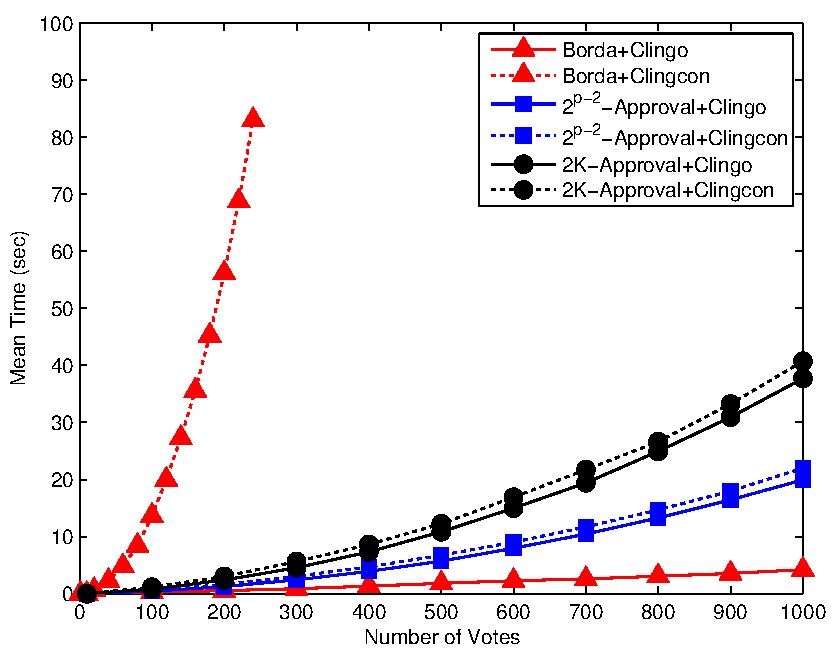
\includegraphics[width=\textwidth]{figs/figs_in_ADT/fixedIssues10SCICP.pdf}
%%		\caption{Winner, fixed \#Issues (10)}
%%		\label{fig:comparison:1}
%%	\end{subfigure}
%%  \begin{subfigure}[b]{0.5\textwidth}
%%		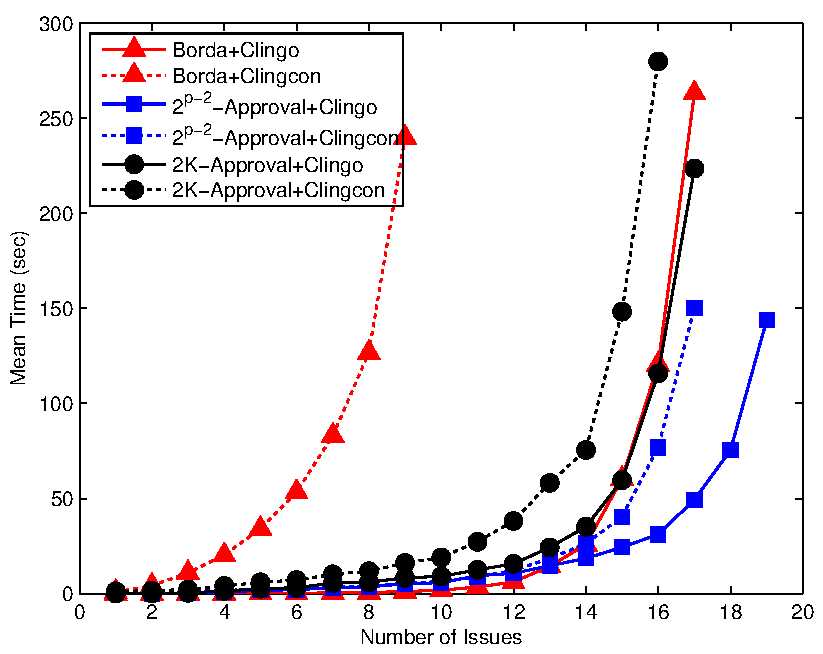
\includegraphics[width=\textwidth]{figs/figs_in_ADT/fixedVotes500SCICP.pdf}
%%    \caption{Winner, fixed \#Votes (500)}
%%		\label{fig:comparison:2}
%%	\end{subfigure}
%%  \\
%%  \begin{subfigure}[b]{0.5\textwidth}
%%		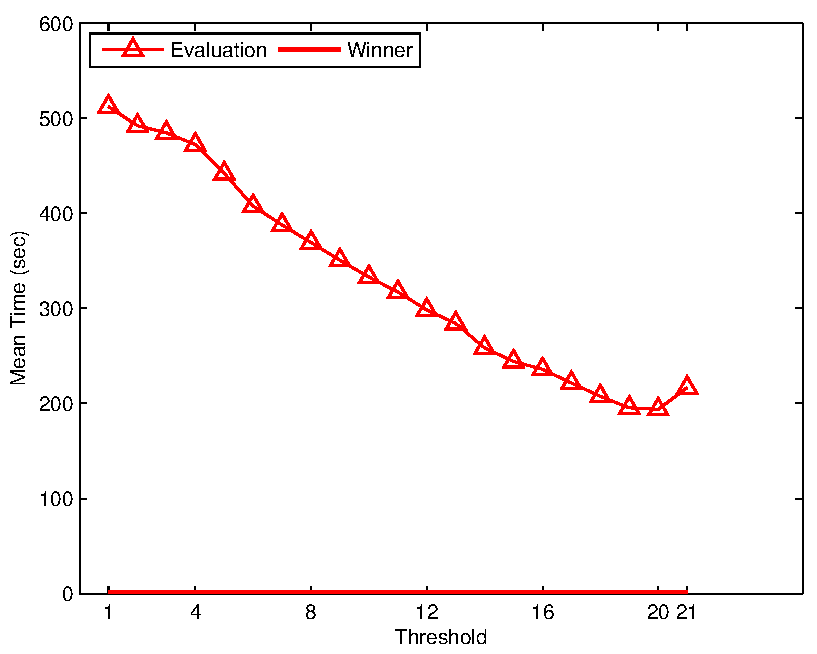
\includegraphics[width=\textwidth]{figs/figs_in_ADT/bordaClingo.pdf}
%%    \caption{Borda, \emph{clingo} (500votes/3attributes)}
%%		\label{fig:comparison:3}
%%	\end{subfigure}
%%  \begin{subfigure}[b]{0.5\textwidth}
%%		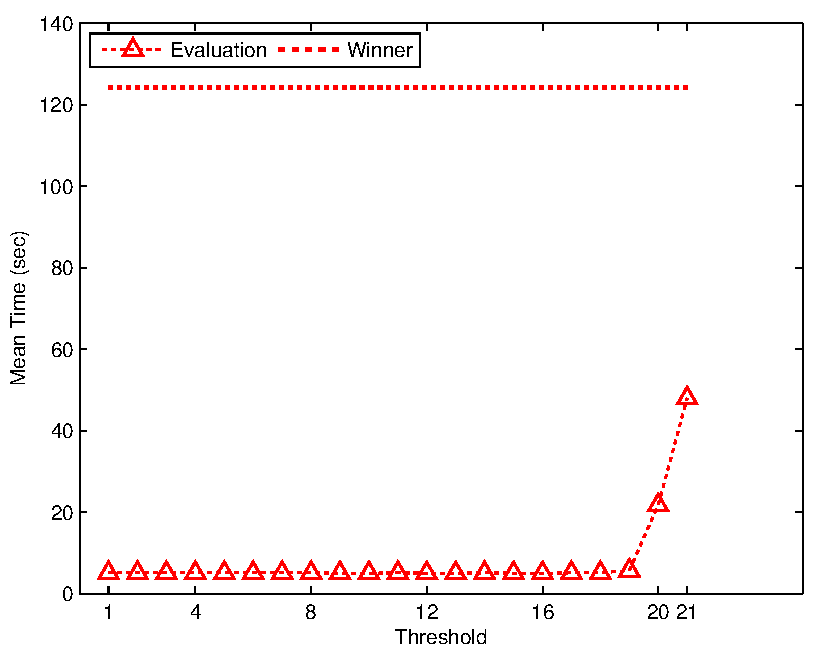
\includegraphics[width=\textwidth]{figs/figs_in_ADT/bordaClingcon.pdf}
%%    \caption{Borda, \emph{clingcon} (500votes/8attributes)}
%%		\label{fig:comparison:4}
%%	\end{subfigure}
%%  \\
%%  \begin{subfigure}[b]{0.5\textwidth}
%%		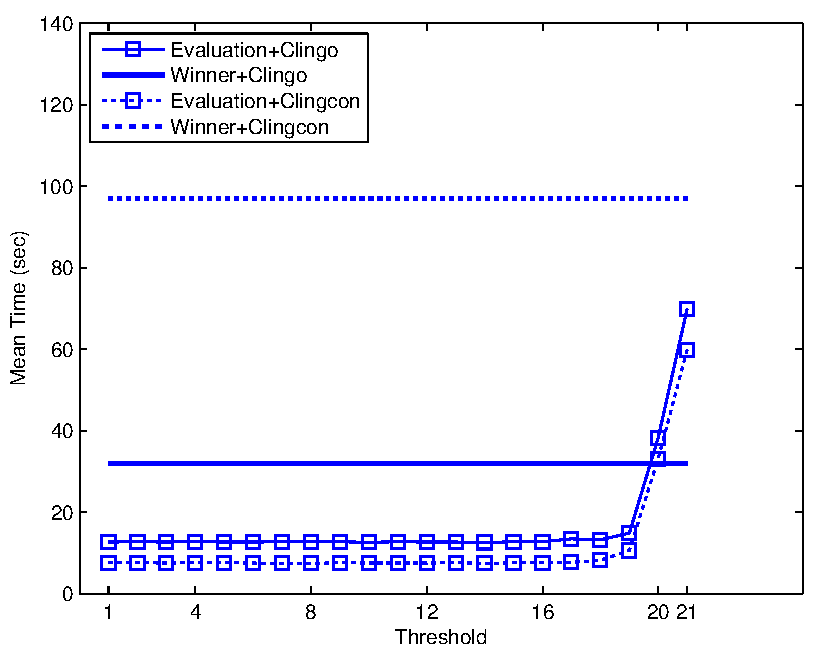
\includegraphics[width=\textwidth]{figs/figs_in_ADT/expAppSCICP.pdf}
%%    \caption{$2^{p-2}$-Approval (500votes/16attributes)}
%%		\label{fig:comparison:5}
%%	\end{subfigure}
%%  \begin{subfigure}[b]{0.5\textwidth}
%%		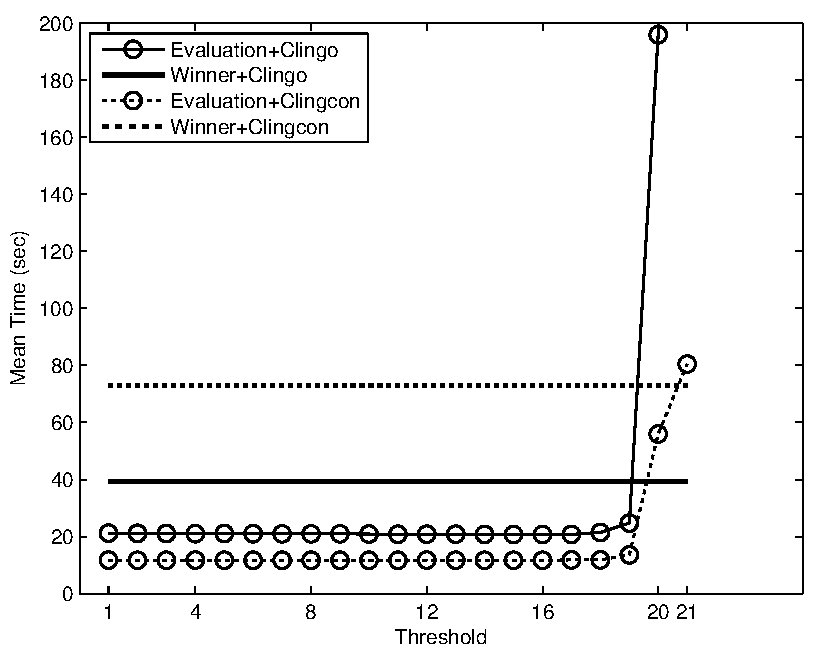
\includegraphics[width=\textwidth]{figs/figs_in_ADT/2kAppSCICP.pdf}
%%    \caption{$2K$-Approval (500votes/14attributes)}
%%		\label{fig:comparison:6}
%%	\end{subfigure}
%%	\end{tabular}
%%  \caption{Aggregating \textit{simple} LP-trees}
%%  \label{fig:comparison}
%%
%%\end{figure*}
%%
%%All our experiments were performed on a machine with an 
%%Intel(R) Core(TM) i7 CPU @ 2.67GHz and 8 GB RAM running 
%%Ubuntu 12.04 LTS.  
%%Each test case (using \emph{clingo 3.0.5} or \emph{clingcon 2.0.3}) was performed with 
%%a limit of 10 minutes.
%%
%%We first consider the winner problem. In the study, we consider the 
%%computation time with a fixed number of attributes (5/10/20) and for each number of attributes we range 
%%the number of votes in a profile up to 1000 for $\{Borda, 2^{p-2}$-$approval, 
%%2K$-$approval\} \times \{clingcon, clingo\}$.  
%%Then we fix the number of votes (500) and vary the number of attributes up to 20, again for 
%%same set of settings.  Each time 
%%result in seconds 
%%is computed as the mean of 10 tests over different randomly generated profiles of 
%%\textit{simple} LP-trees.
%%
%%For the evaluation problem, we compare its experimental complexity with that of the winner problem.
%%For each of the 10 randomly generated profiles, we compute the winning score 
%%$\WS$ 
%%and set the threshold for the evaluation problem with a percentage of $\WS$, starting with 
%%$5\%$ and incremented by $5\%$ for the following tests until we reach the full
%%value of $\WS$. We run one more test with the threshold $\WS+1$ (there is 
%%no solution then and the overall method allows for the experimental 
%%comparison of the hardness of the winner and evaluation problems).
%%That allows us to study the effectiveness of the maximization construct in
%%\emph{clingo} (the main difference between the \emph{winner} and the 
%%\emph{evaluation} problems is in the use of that construct in the 
%%encoding of the former).
%%We again present and compare average time results.
%%
%%\subsubsection{Varying the number of attributes and the number of votes}
%%%$p$ and $n$}
%%Our experiments on the winner problem for the three voting rules with 
%%the fixed number of attributes are consistent with the property that the problem
%%is solvable in polynomial time. 
%%Both \emph{clingo} and \emph{clingcon} scale up well.
%%\figref{comparison:1} depicts the results for the cases with 
%%10 attributes. When we fix the number of votes and vary the number of 
%%attributes the time grows exponentially with $p$ (cf. \figref{comparison:2}),
%%again consistently with the computational complexity of the problems
%%(NP-hardness).
%%
%%Generally \emph{clingo} is better compared to \emph{clingcon} in solving 
%%the winner problem for the three scoring rules. We attribute that first 
%%to the use of the optimization construct in \emph{clingo}, which allows
%%us to keep the size of the ground propositional theory low, and second to 
%%the effective way in which optimization constructs are implemented in that 
%%system. Thus, in these examples, the main benefit of \emph{clingcon},
%%its ability to avoid grounding and preprocessing by ``farming out'' some of the solving job
%%to a dedicated constraint solver, does not offer \emph{clingcon} the edge.
%%Finally, for both \emph{clingo} and \emph{clingcon}, Borda is the hardest
%%rule to deal with, especially when the number of attributes is large.
%%
%%\subsubsection{Comparison of the problems: evaluation vs winner}
%%
%%The evaluation problem can be reduced to the winner problem, as
%%an evaluation problem instance has an answer \textit{YES}
%%if and only if the score of the winner equals or exceeds the threshold.
%%Thus, the evaluation problem is at most as complex as
%%the winner problem.
%%
%%We compared the two problems by first solving the winner problem, and then
%%solving the evaluation problem on the same instances with the value of
%%the threshold growing at the step of 5\% of the winner score. That gives us
%%20 normalized points for each instance. In the last run (point 21 on the
%%$x$-axis) we used the winner's score plus 1 as the threshold to determine
%%the optimality of the winner's score. These experiments allow us to compare
%%the hardness of the winner problem (more precisely, the effectiveness 
%%of solvers) with that of the evaluation problem. 
%%
%%First, we note that for \emph{clingo}, the evaluation problem is
%%harder than the winner problem in the entire range for Borda ( 
%%\figref{comparison:3}), and for the two other rules, when the threshold 
%%is close to the winner's score or exceeds it (\figref{comparison:5}
%%and \figref{comparison:6}). We attribute that to the fact that the encodings 
%%of the evaluation problem have to model the threshold constraint with the 
%%\textit{\#sum} rule which, in \emph{clingo}, leads to large ground theories 
%%that it finds hard to handle. In the winner problem encodings, the \textit{\#sum} 
%%rule is replaced with an optimization construct, which allows us to keep
%%the size of the ground theory low.
%%
%%For \emph{clingcon} the situation is different. 
%%\figref{comparison:4}, \figref{comparison:5} and \figref{comparison:6}
%%show that the evaluation problem is easier than the winner problem
%%when the threshold values are smaller than the winning score and 
%%the evaluation problem becomes harder when the thresholds are close to it.
%%It seems to suggest that the constraint solver used by \emph{clingcon} 
%%performs well in comparison with the implementation of the optimization 
%%constructs in \emph{clingcon}.
%%Finally, in all cases \emph{clingcon} outperforms \emph{clingo} on the
%%evaluation problems. It is especially clear for Borda, where the range of
%%scores is much larger than in the case of approval rules. That poses a
%%challenge for \emph{clingo} that instantiates the \textit{\#sum} rule over
%%that large range, which \emph{clingcon} is able to avoid.

\section{Experiments}
Here we present and analyze the experimental results from solving the Winner problem
and the Evaluation problem using two Answer Set Programming solvers
$\clingo$ (version 4.2.1) and $\clingcon$ (version 2.0.3)
and one Constraint Satisfaction Problem solver $\toulbar$ (version 0.9.6.0-dev).

All our experiments were performed on a machine with an 
Intel(R) Core(TM) i7 CPU @ 2.67GHz and 8 GB RAM running 
Ubuntu 12.04 LTS.  

We first consider the winner problem. In the study, we consider the 
computation time with a fixed number of attributes (5/10/20) and for each number of attributes we range 
the number of votes in a profile up to 3000 for $\{Borda, 2^{p-2}$-$approval, 
2K$-$approval\} \times \{\clingcon, \clingo, \toulbar\}$.  
Then we fix the number of votes (1000) and vary the number of attributes up to 20, again for 
same set of settings.  Each time 
result in seconds 
is computed as the mean of 20 tests over different randomly generated profiles of 
LP-trees.

\subsection{Structure of the Simple LP Trees}
To experiment with the programs presented above and with \emph{clingo} and
\emph{clingcon} solvers, we generate logic programs that represent 
random LP-trees and profiles of random
LP-trees.
Our algorithm generates encodings of trees from the most general class CI-CP 
under the following restrictions:
(1) Each LP-tree has exactly two paths with the splitting node appearing 
at depth $d_s=\left \lfloor \frac{p}{2} \right \rfloor$;
(2) Each non-root node at depth $\leq d_s+1$ has exactly one parent;
(3) Each 
node at depth $> d_s+1$ has exactly two parents, one of which 
is at depth $< d_s$.\footnote{
The restrictions are motivated by the size of the representation
considerations. They ensure that the size of generated LP-trees is 
linear in the number of attributes.}

The algorithm starts by randomly selecting attributes to label the nodes on 
the path from the root to the splitting node and then, similarly, labels 
the nodes on each of the two paths (different labeling can be produced
for each of them). Then, for each non-root node, the algorithm selects at random
one or two parent nodes (as appropriate based on the location of the node).
Finally, the algorithm decides 
local preferences (for each combination of values of the parent attributes)
randomly picking one over the other. In each step, all 
possible choices are equally likely. We call CI-CP LP-trees satisfying 
these restrictions \emph{simple}. Each simple LP-tree has size 
linear in $p$.  \figref{MSCICP_tree} depicts a CI-CP tree of 
4 attributes in this class. 
\begin{figure}
\centering
	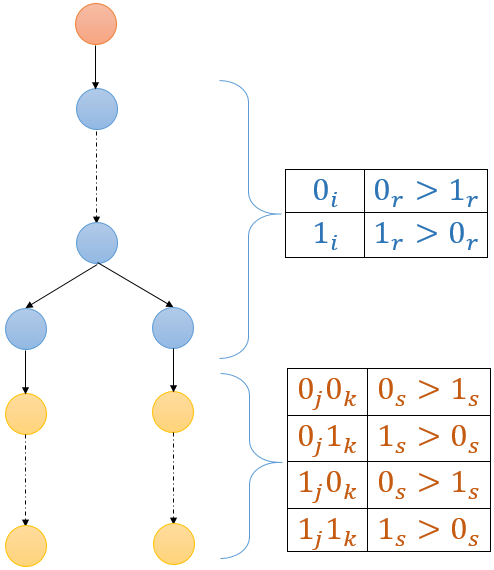
\includegraphics[width=0.5\textwidth]{img/simple_LP_tree.png}
\caption{\emph{Simple} CI-CP tree}
\label{fig:MSCICP_tree}
\end{figure}



\subsection{Solving the Winner Problem}

We refer to \ref{fig:win} for the empirical results on solving the Winner problem.  
Each point in a figure represents
an average of computation time spent on solving 20 different 
Winner problem instances given randomly
generated LP profiles.

\begin{figure*}[ht!]
	\centering
	\setlength{\tabcolsep}{0mm}
	\begin{tabular}{c}
  \begin{subfigure}[b]{0.44\textwidth}
		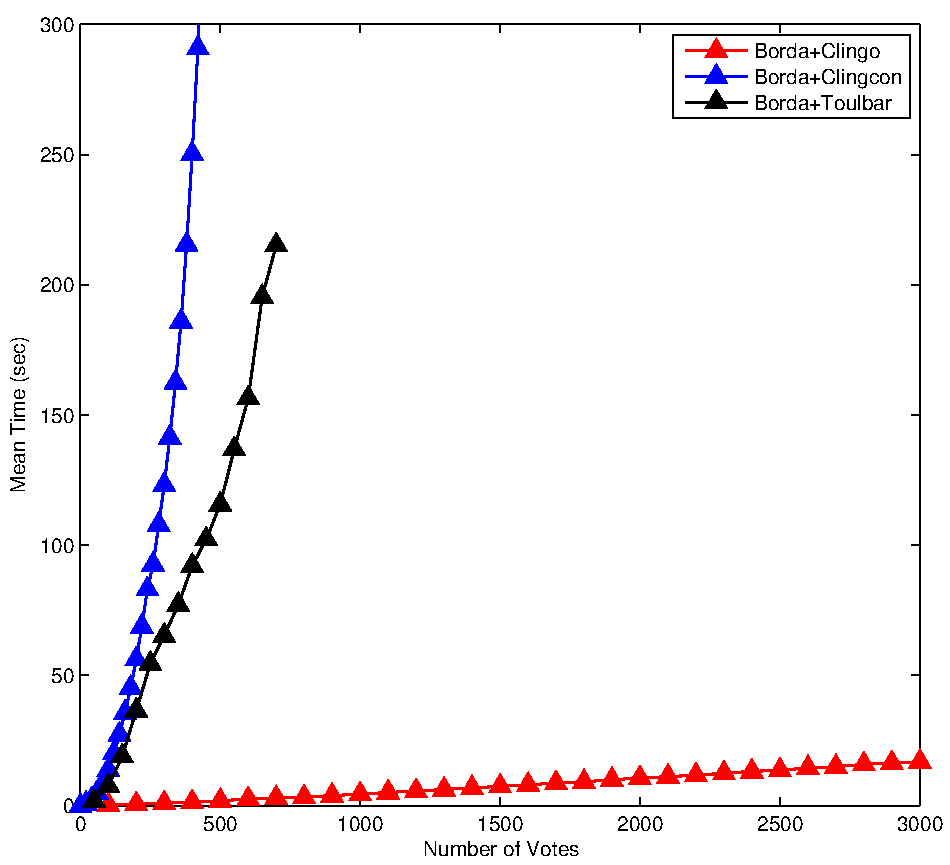
\includegraphics[width=\textwidth]{figs/bordaFIMSCICP.pdf}
		\captionsetup{font=scriptsize}
		\caption{Borda, fixed \#attributes(10)}
		\label{fig:comparison:win:1}
	\end{subfigure}
  \begin{subfigure}[b]{0.44\textwidth}
		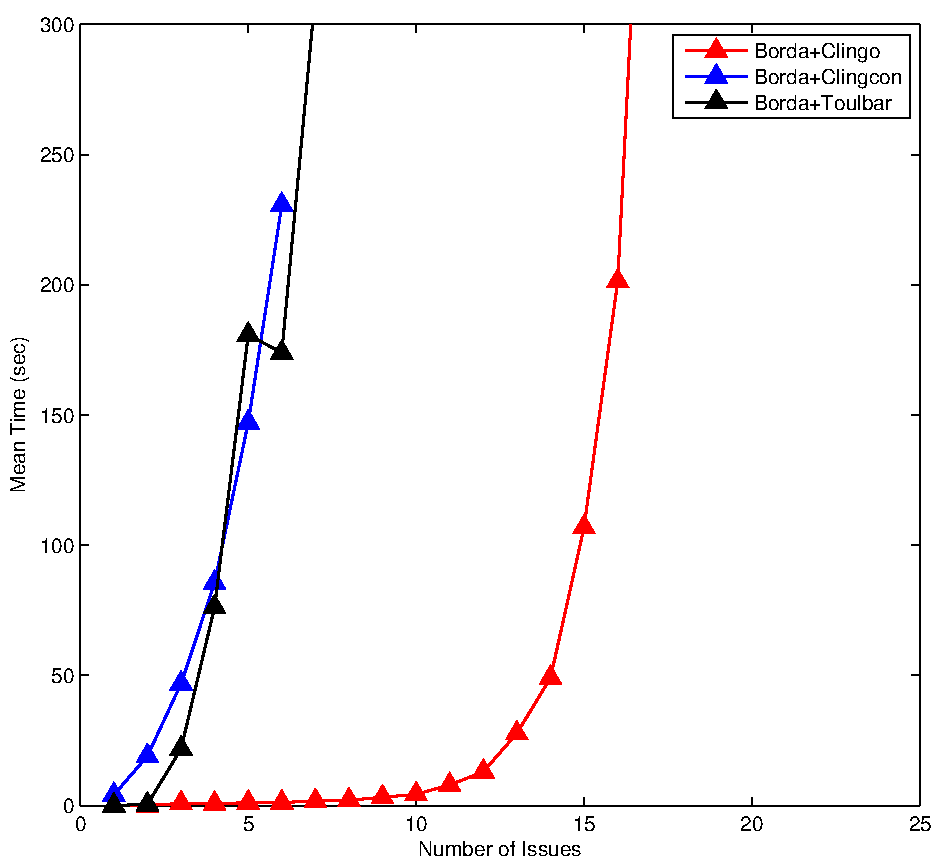
\includegraphics[width=\textwidth]{figs/bordaFVMSCICP.pdf}
		\captionsetup{font=scriptsize}
    \caption{Borda, fixed \#votes(1000)}
		\label{fig:comparison:win:2}
	\end{subfigure}
  \\
  \begin{subfigure}[b]{0.44\textwidth}
		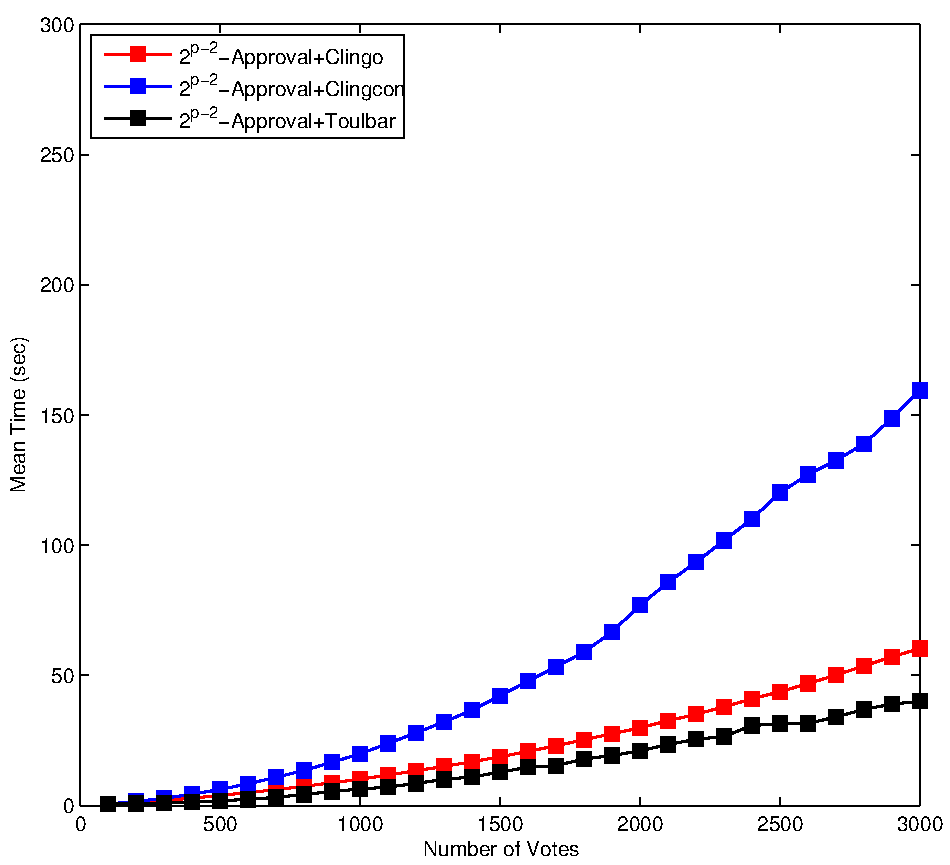
\includegraphics[width=\textwidth]{figs/expAppFIMSCICP.pdf}
		\captionsetup{font=scriptsize}
    \caption{$2^{p-2}$-Approval, fixed \#attributes(10)}
		\label{fig:comparison:win:3}
	\end{subfigure}
  \begin{subfigure}[b]{0.44\textwidth}
		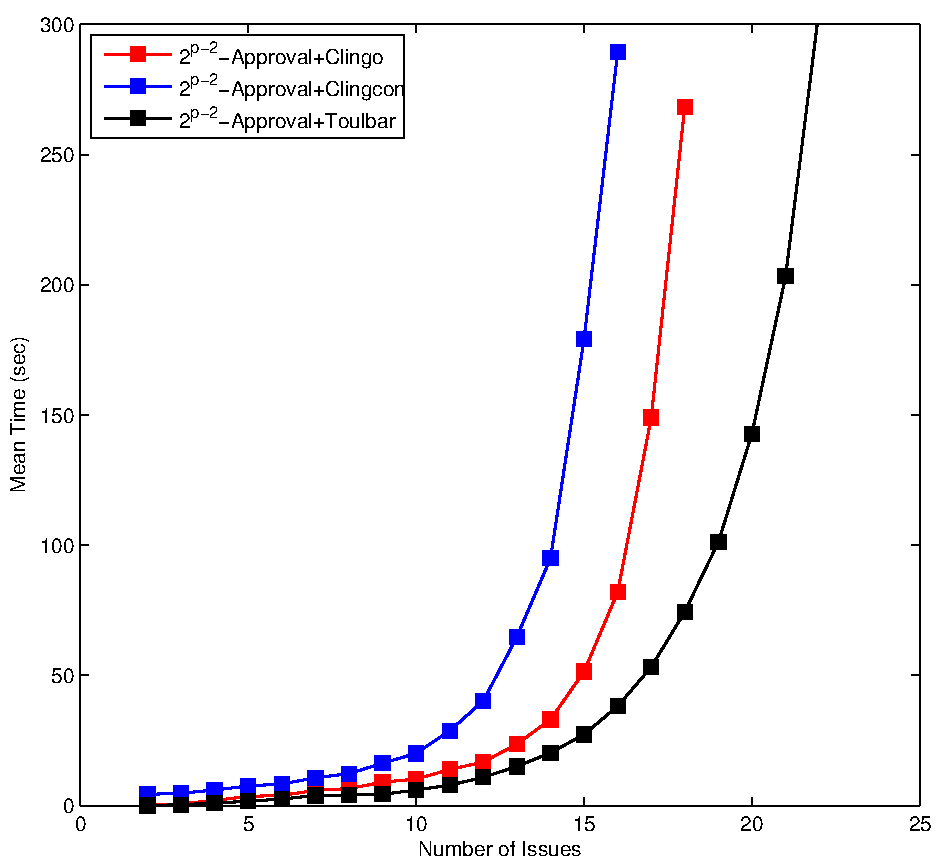
\includegraphics[width=\textwidth]{figs/expAppFVMSCICP.pdf}
		\captionsetup{font=scriptsize}
    \caption{$2^{p-2}$-Approval, fixed \#votes(1000)}
		\label{fig:comparison:win:4}
	\end{subfigure}
  \\
  \begin{subfigure}[b]{0.44\textwidth}
		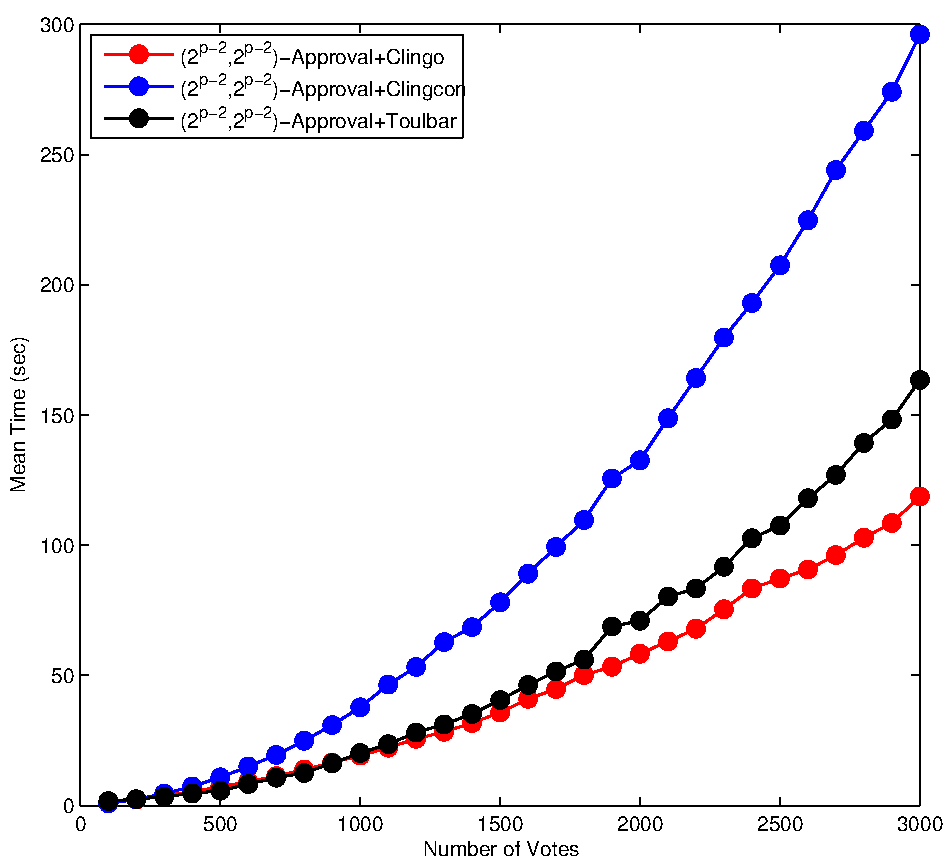
\includegraphics[width=\textwidth]{figs/2kAppFIMSCICP.pdf}
		\captionsetup{font=scriptsize}
    \caption{$2K$-Approval, fixed \#attributes(10)}
		\label{fig:comparison:win:5}
	\end{subfigure}
  \begin{subfigure}[b]{0.44\textwidth}
		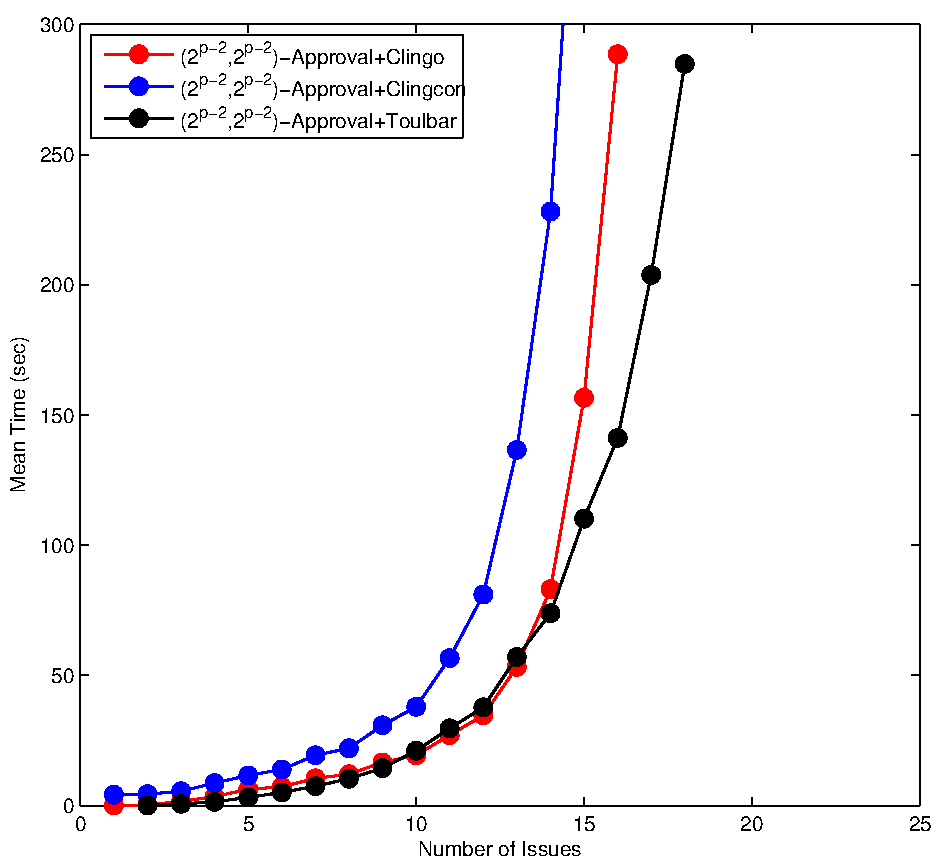
\includegraphics[width=\textwidth]{figs/2kAppFVMSCICP.pdf}
		\captionsetup{font=scriptsize}
    \caption{$2K$-Approval, fixed \#votes(1000)}
		\label{fig:comparison:win:6}
	\end{subfigure}
	\end{tabular}
  \caption{Solving the winner problem given \textit{simple} LP-trees}
  \label{fig:win}

\end{figure*}


It is clear that our experiments on the winner problem for the three voting rules with 
fixed number of attributes are consistent with the property that the problem
is solvable in polynomial time. All three solvers scale up well.
Figures \ref{fig:win}(a),(c) and (e) depict the result for the cases with 10 attributes.
When we fix the number of votes and vary the number of 
attributes the time grows exponentially with $p$ (cf. Figures \ref{fig:win}(b),(d) and (f)),
again consistently with the computational complexity of the problems (NP-hardness).

Generally $\clingo$ is better compared to $\clingcon$ in solving 
the winner problem for the three scoring rules. Moreover,
$\clingo$ outperforms $\toulbar$ in solving the winner problem for
the Borda rule, while $\toulbar$ performs better than $\clingo$
for the two approval rules.

For the winner problems, our experiments demonstrates that profiles
of LP-trees of practical sizes can be effectively handled by our
solvers, up to 3000 votes per profile over up to 20 attributes.
But going beyond 20 attributes remains a challenge.


%%\begin{figure*}[!ht]
%%	\centering
%%	\subfigure[Borda, fixed \#Issues (10)]{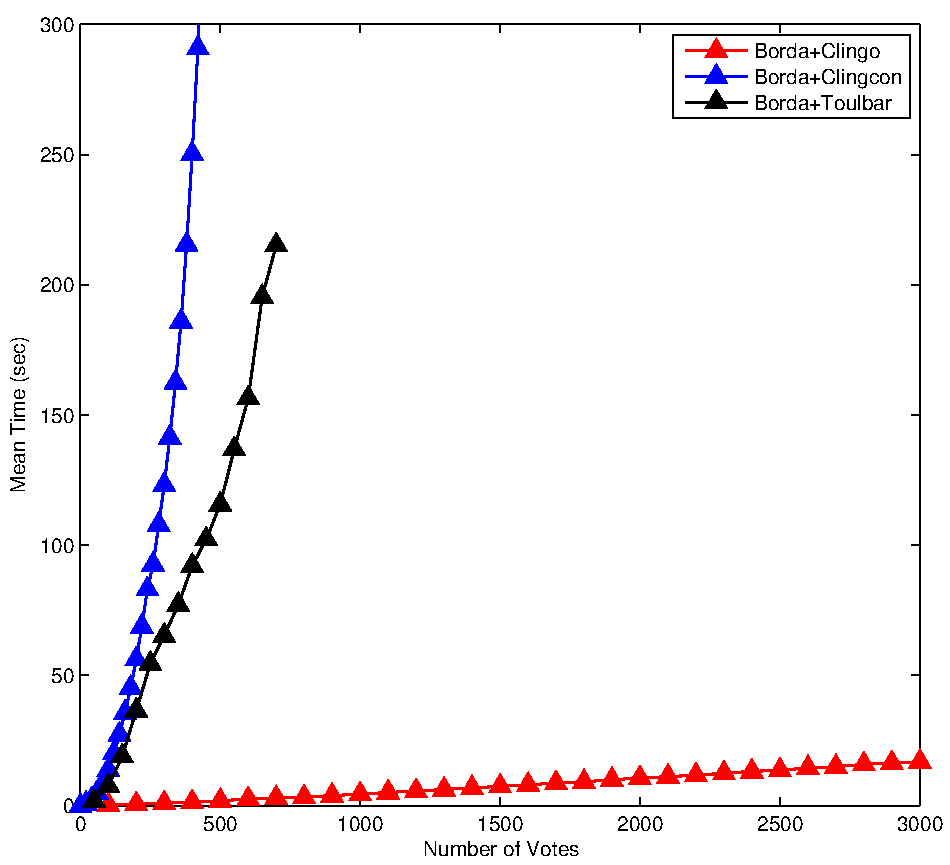
\includegraphics[width=0.45\textwidth]{figs/bordaFIMSCICP.pdf}}%
%%	\subfigure[Borda, fixed \#Votes (1000)]{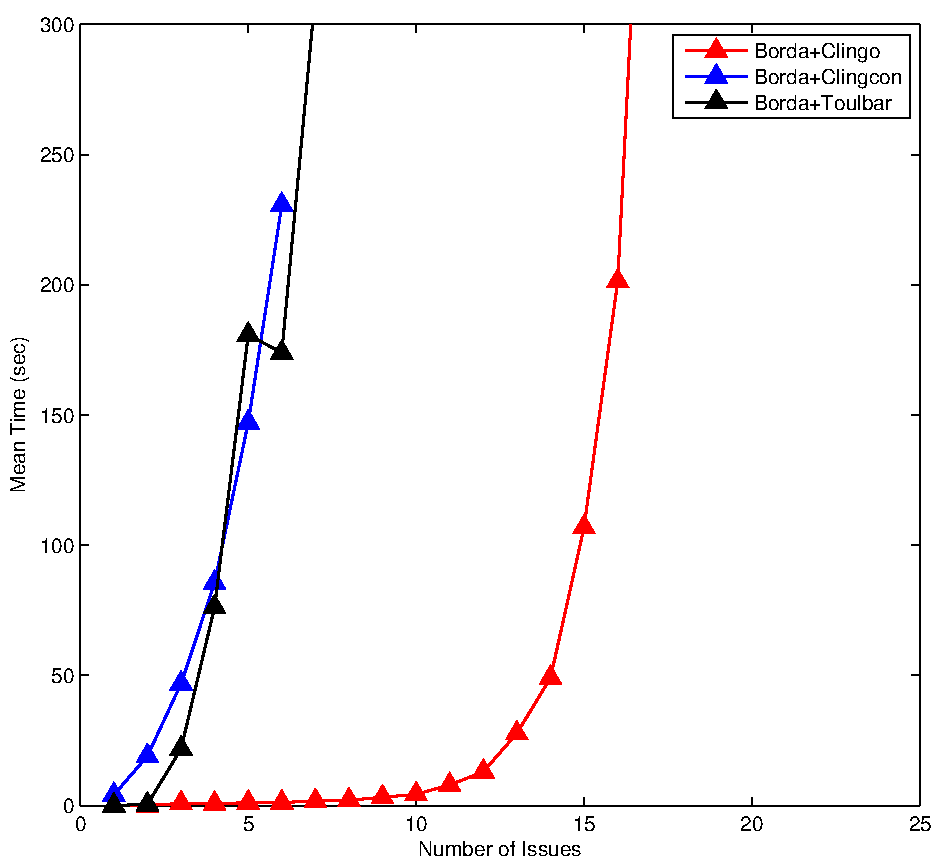
\includegraphics[width=0.45\textwidth]{figs/bordaFVMSCICP.pdf}} \\
%%	\subfigure[$2^{p-2}$-Approval, fixed \#Issues (10)]{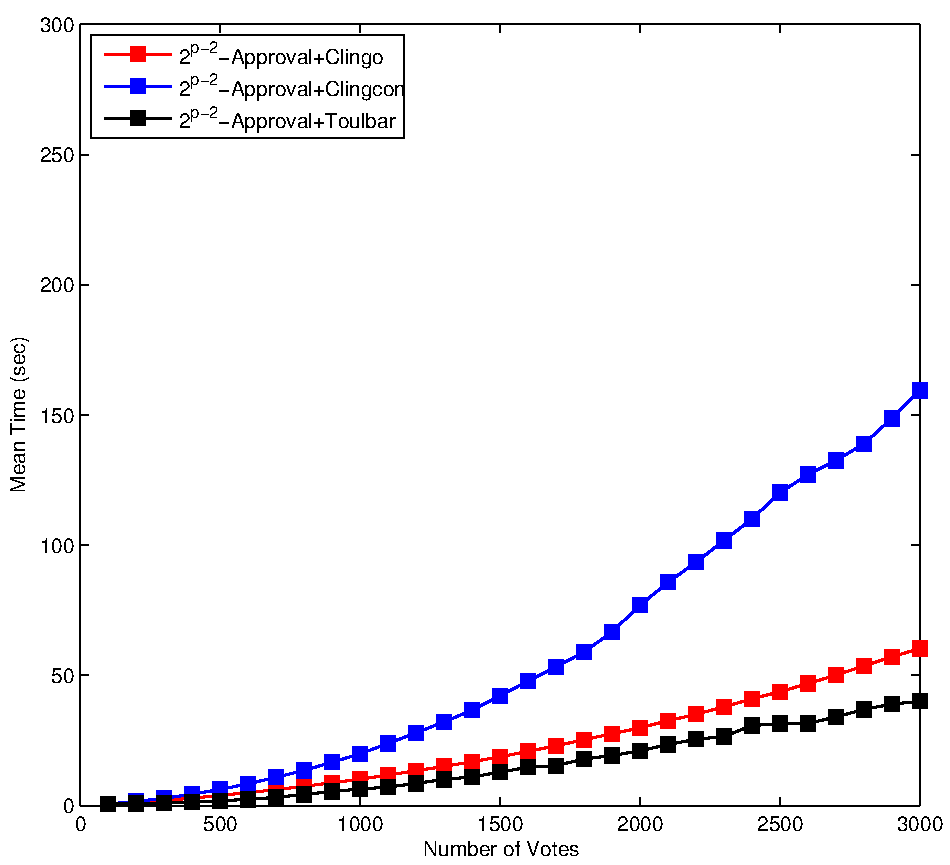
\includegraphics[width=0.45\textwidth]{figs/expAppFIMSCICP.pdf}}%
%%	\subfigure[$2^{p-2}$-Approval, fixed \#Votes (1000)]{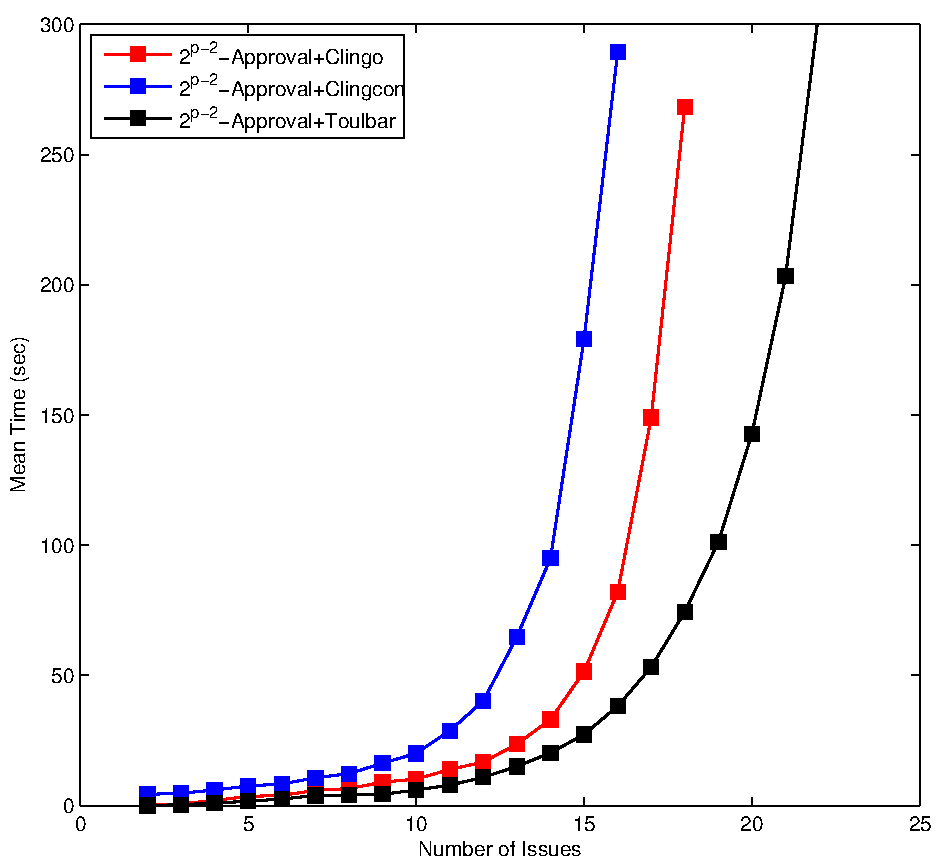
\includegraphics[width=0.45\textwidth]{figs/expAppFVMSCICP.pdf}} \\
%%	\subfigure[$2K$-Approval, fixed \#Issues (10)]{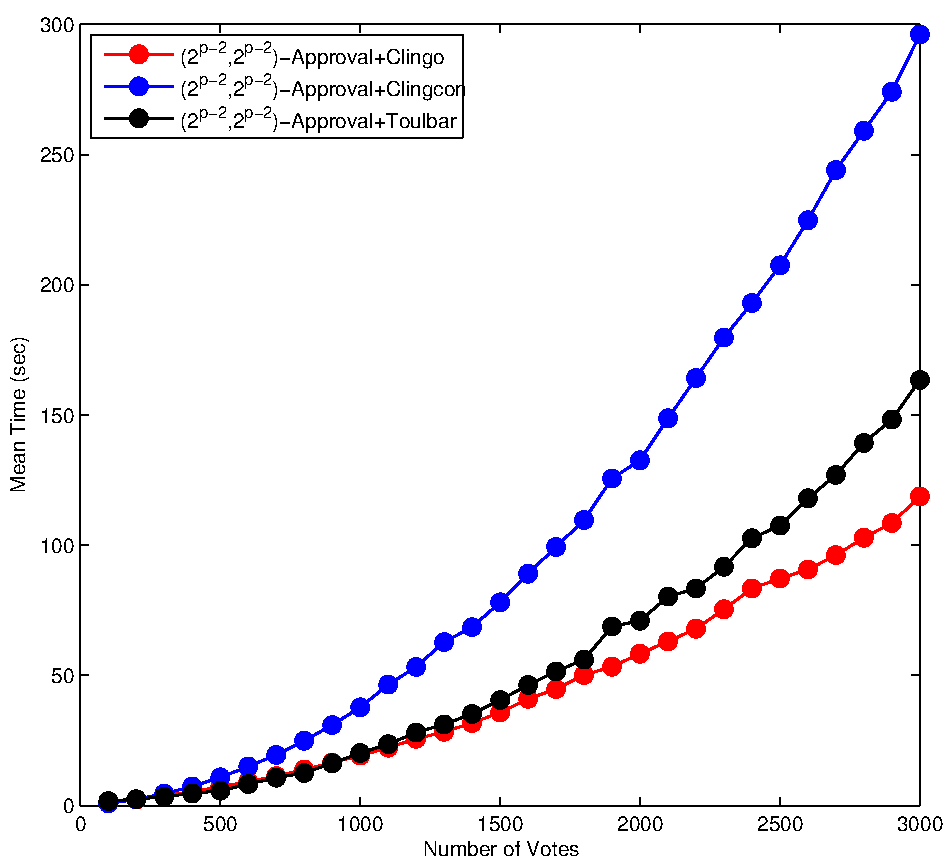
\includegraphics[width=0.45\textwidth]{figs/2kAppFIMSCICP.pdf}}%
%%	\subfigure[$2K$-Approval, fixed \#Votes (1000)]{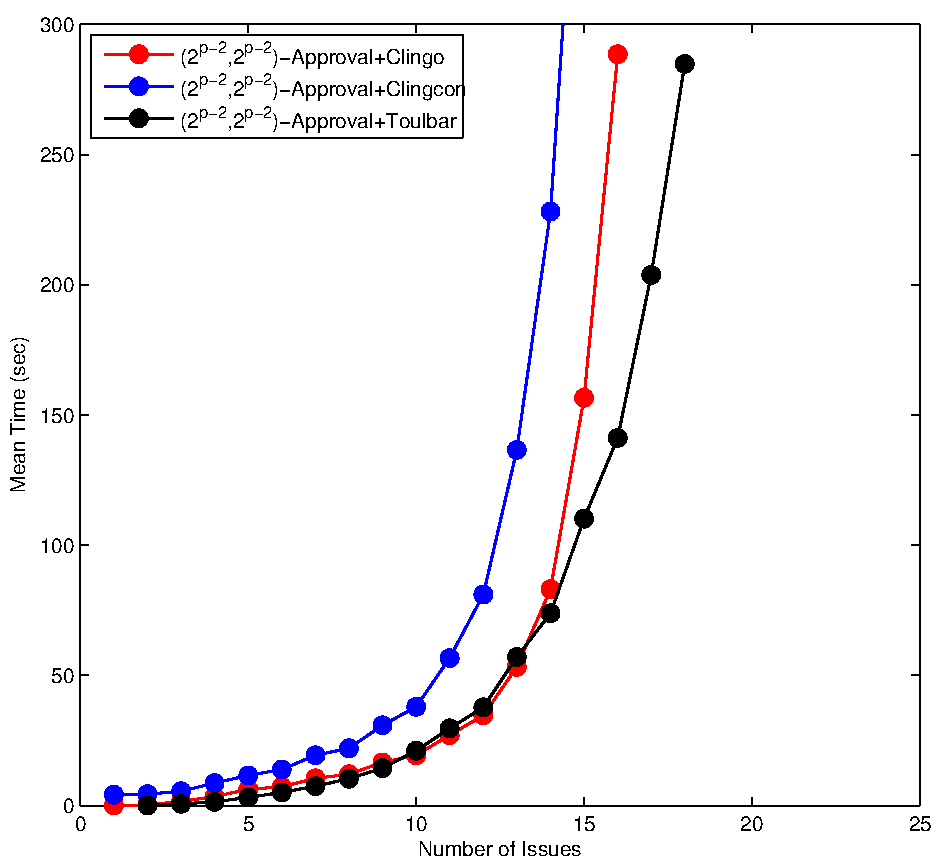
\includegraphics[width=0.45\textwidth]{figs/2kAppFVMSCICP.pdf}}
%%
%%  \caption{Solving the winner problem given \textit{simple} LP-trees}
%%  \label{fig:win}
%%
%%\end{figure*}



\subsection{Solving the Evaluation Problem}
The evaluation problem can be reduced to the winner problem, as
an evaluation problem instance has an answer \textit{YES}
if and only if the score of the winner equals or exceeds the threshold.
Thus, the evaluation problem is at most as complex as
the winner problem.

%%\begin{figure*}[!ht]
%%	\centering
%%	\subfigure[$2^{p-2}$-Approval (1000votes/13attributes)]{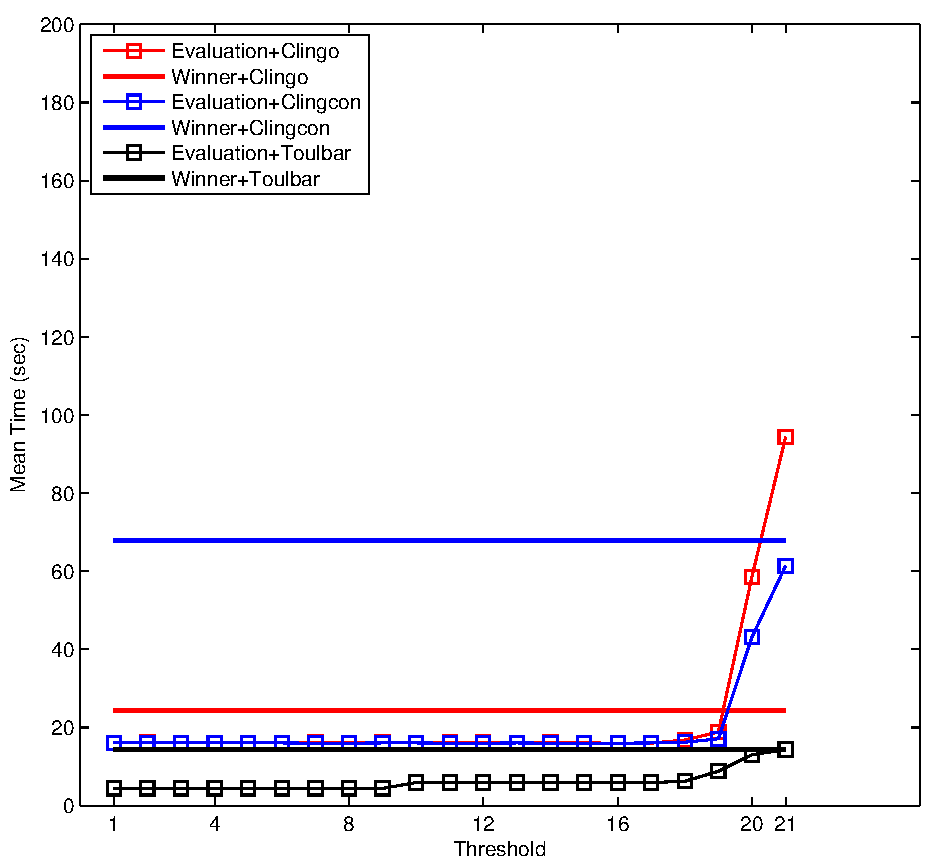
\includegraphics[width=0.45\textwidth]{figs/expAppMSCICP_1000v_13i.pdf}}%
%%	\subfigure[$2K$-Approval (1000votes/13attributes)]{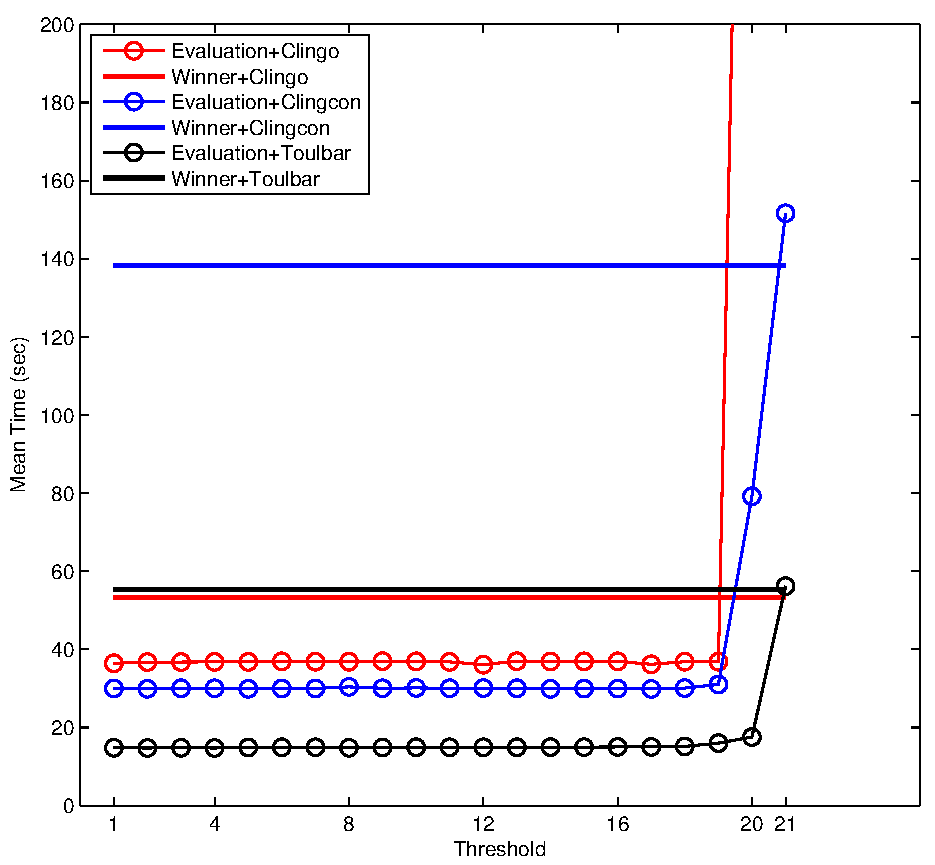
\includegraphics[width=0.45\textwidth]{figs/2kAppMSCICP_1000v_13i.pdf}}\\
%%	\subfigure[Borda (1000votes/4attributes)]{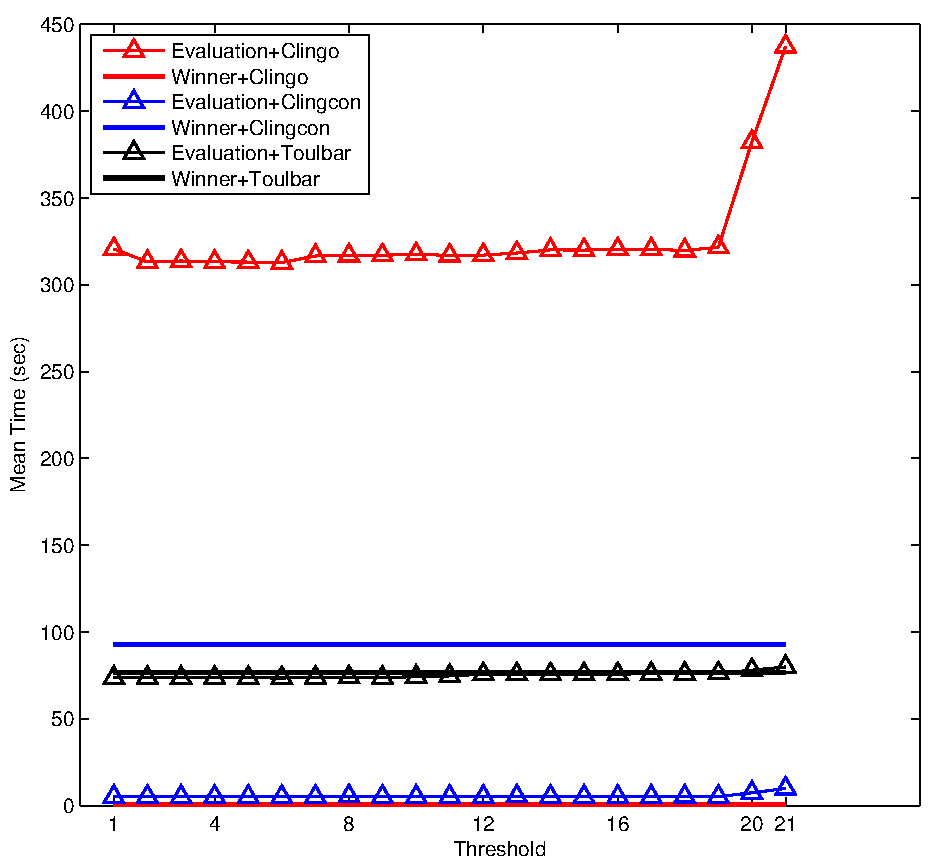
\includegraphics[width=0.45\textwidth]{figs/bordaMSCICP_1000v_4i.pdf}}
%%
%%  \caption{Solving the evaluation problem given \textit{simple} LP-trees}
%%  \label{fig:eval}
%%
%%\end{figure*}

\begin{figure*}[!ht]
	\centering
	\setlength{\tabcolsep}{0mm}
	\begin{tabular}{c}
  \begin{subfigure}[b]{0.5\textwidth}
		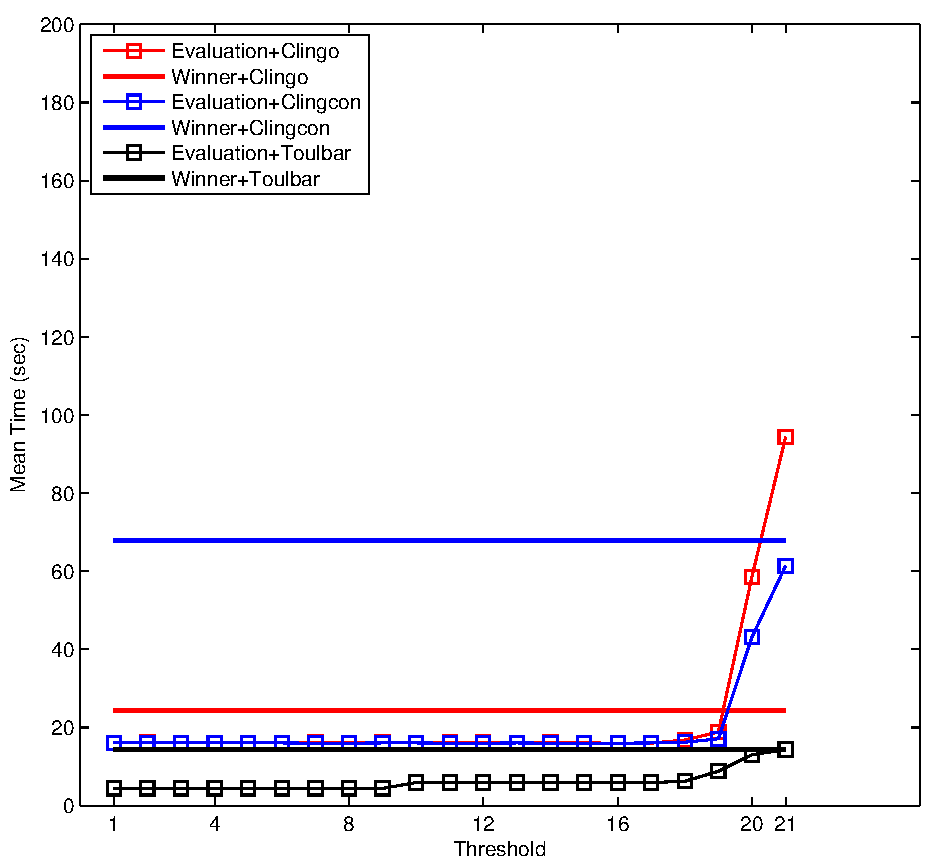
\includegraphics[width=\textwidth]{figs/expAppMSCICP_1000v_13i.pdf}
		\captionsetup{font=scriptsize}
		\caption{$2^{p-2}$-Approval (1000votes/13attributes)}
		\label{fig:comparison:eval:1}
	\end{subfigure}
  \begin{subfigure}[b]{0.5\textwidth}
		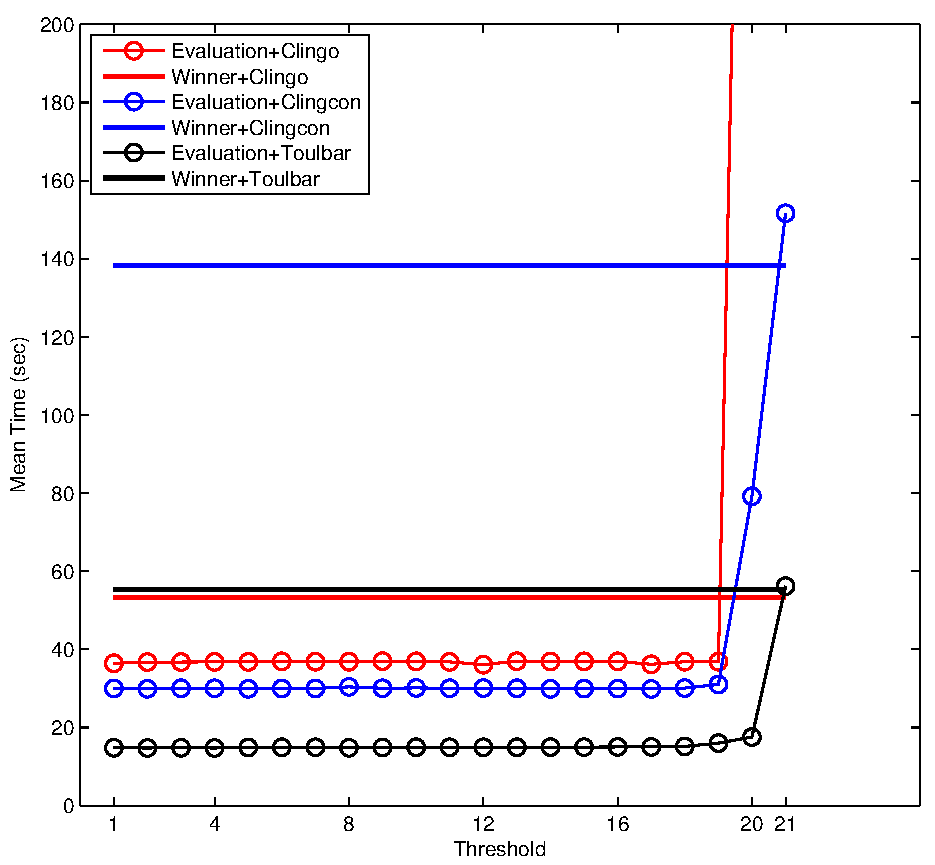
\includegraphics[width=\textwidth]{figs/2kAppMSCICP_1000v_13i.pdf}
		\captionsetup{font=scriptsize}
    \caption{$2K$-Approval (1000votes/13attributes)}
		\label{fig:comparison:eval:2}
	\end{subfigure}
  \\
  \begin{subfigure}[b]{0.5\textwidth}
		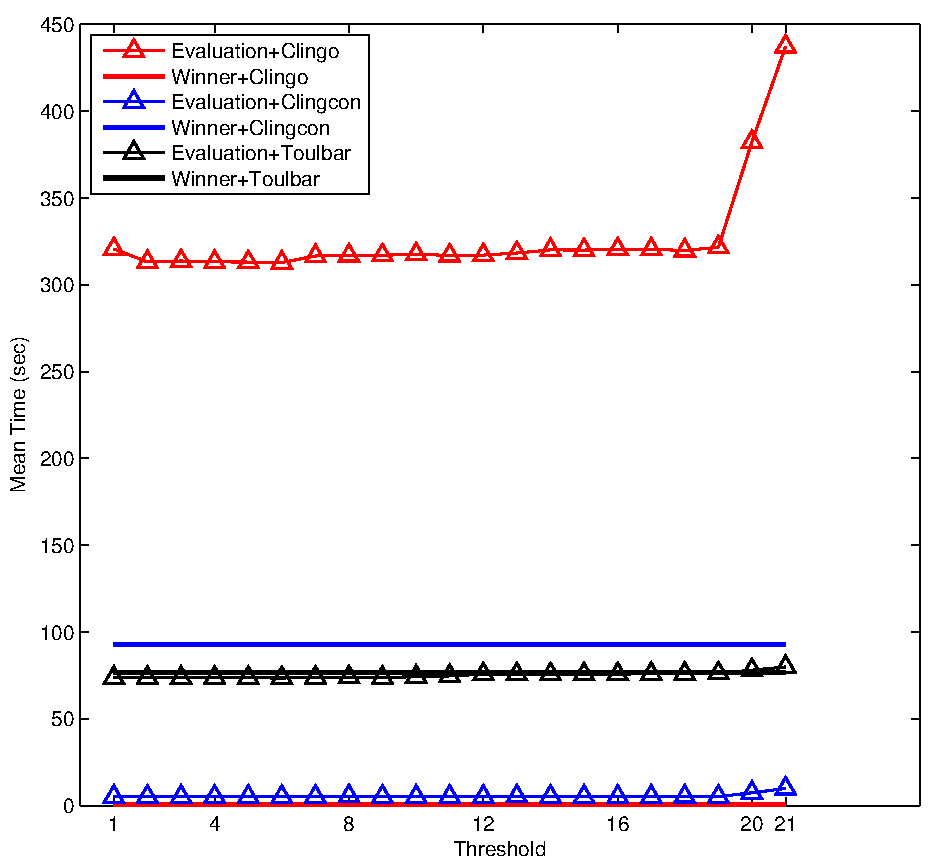
\includegraphics[width=\textwidth]{figs/bordaMSCICP_1000v_4i.pdf}
		\captionsetup{font=scriptsize}
    \caption{Borda (1000votes/4attributes)}
		\label{fig:comparison:eval:3}
	\end{subfigure}
	\end{tabular}
  \caption{Solving the evaluation problem given \textit{simple} LP-trees}
  \label{fig:eval}
\end{figure*}

For the evaluation problem, we compare its experimental complexity with
that of the winner problem. For each of the $20$ randomly generated profiles
of 1000 votes, we
compute the winning score $\WS$ and set the threshold for the evaluation problem
with a percentage of $\WS$, starting with $5\%$ and incremented by $5\%$ for the
following tests until we reach the full value of $\WS$. We run one more test with the
threshold $\WS +1$ (there is no solution then and the overall method allows for the
experimental comparison of the hardness of the winner and evaluation problems).
That allows us to study the effectiveness of solvers. We again present and
compare average time results.

First, we note that for $\clingo$, the evaluation problem is
harder than the winner problem in the entire range for Borda (\figref{eval}(c)).
We attribute that to the fact that the encodings 
of the evaluation problem have to model the threshold constraint with the 
\textit{\#sum} rule which, in $\clingo$, leads to large ground theories 
that it finds hard to handle. In the winner problem encodings, the \textit{\#sum} 
rule is replaced with an optimization construct, which allows us to keep
the size of the ground theory low.

Second, we notice that, except for Borda and $\clingo$,
the evaluation problem is easier than the winner problem
when the threshold values are smaller than the winning score and 
the evaluation problem becomes harder when the thresholds are close to it.
We refer to Figures \ref{fig:eval}(a), (b) and (c).

Thirdly, in all cases \emph{clingcon} outperforms \emph{clingo} on the
evaluation problems (cf. Figures \ref{fig:eval}(a), (b) and (c)). 
It is especially clear for Borda, where the range of
scores is much larger than in the case of approval rules. That poses a
challenge for \emph{clingo} that instantiates the \textit{\#sum} rule over
that large range, which \emph{clingcon} is able to avoid.

Finally, we compare the effectiveness of $\clingcon$ and $\toulbar$ on
solving the evaluation problems. Generally, $\clingcon$ performs better
for the Borda rule, whereas $\toulbar$ is better for the two approval rules.
Again, to see this, we refer to Figures \ref{fig:eval}(a), (b) and (c).


\section{Conclusions}
Aggregating votes expressed as LP-trees is a rich source of interesting
theoretical and practical problems. In particular, the complexity of the
winner and evaluation problems for scoring rules is far from
being fully understood. First results on the topic were provided by 
Lang et al. \cite{lang:aggLP}; our work exhibited another class of positional
scoring rules for which the problems are NP-hard and NP-complete, 
respectively. However, a full understanding of what makes a positional 
scoring rule hard remains an open problem.

Importantly, our results show that ASP tools are effective in modeling 
and solving the winners and the evaluation problems for some positional 
scoring rules such as Borda, $2^{p-2}$-approval and $2K$-approval. When 
the number of attributes is fixed the ASP tools scale up consistently with 
the polynomial time complexity. In general, the tools are practical even 
if the number of attributes is up to 15 and the number of votes is as high 
as 500. This is remarkable as 15 binary attributes determine the space of over 
30,000 alternatives. 

Finally, the preference aggregation problems form 
interesting benchmarks for ASP tools that stimulate advances in ASP
solver development. As the preference aggregation problems involve large 
domains, they put to the test those features of ASP tools that attempt 
to get around the problem of grounding programs over large domains. Our 
results show that the optimization statements in \emph{clingo} in 
general perform well. When they cannot be used, as in the evaluation 
problem, it is no longer the case. The solver \emph{clingcon}, which 
reduces grounding and preprocessing work by delegating some tasks to a constraint solver, 
performs well in comparison to \emph{clingo} on the evaluation problem,
especially for the Borda rule (and we conjecture, for all rules that
result in large score ranges).

In the future work we will expand our experimentation by developing
methods to generate richer classes of randomly generated LP-trees.
We will also consider the use of ASP tools to aggregate votes given in
other preference systems such as CP-nets \cite{bbdh03} and answer set 
optimization (ASO) preferences \cite{Brewka:ASO}.
